\documentclass{ociamthesis}

\usepackage{graphicx}
\usepackage[utf8]{inputenc}
\usepackage[T1]{fontenc}
\usepackage{lmodern}
\usepackage[english]{babel}
\usepackage{amsmath}
\usepackage{amsthm}
\usepackage{mathtools}
\usepackage{amssymb}
\usepackage{listings}
\usepackage{xparse}
\usepackage{stmaryrd}
\usepackage{geometry}
\usepackage{enumerate}
\usepackage{tikz}
\usepackage{stmaryrd}
\usepackage{hyperref}
\usepackage{algorithm}
\usepackage{enumitem}
\usepackage[noend]{algpseudocode}
\usepackage[style=english]{csquotes}

\hypersetup{
    colorlinks,
    linkcolor={red!50!black},
    citecolor={blue!50!black},
    urlcolor={blue!80!black}
}

\usetikzlibrary{babel, positioning, shapes.geometric, arrows, arrows.meta}

\title{Generating supersingular curves with modular polynomials}

\author{Simon Pohmann}
\college{St Hugh's College}
\degree{Master of Science in Mathematics}
\degreedate{2022} 

\newcommand{\Z}{\mathbb{Z}}
\newcommand{\Q}{\mathbb{Q}}
\newcommand{\F}{\mathbb{F}}
\newcommand{\C}{\mathbb{C}}
\newcommand{\End}{\mathrm{End}}
\newcommand{\Quot}{\mathrm{Quot}}
\newcommand{\Half}{\mathcal{H}}
\newcommand{\Lattice}{\mathcal{L}}
\newcommand{\divides}{\ \mid \ }
\newcommand{\notdivides}{\ \nmid \ }
\newcommand{\Cl}{\mathrm{Cl}}
\newcommand{\q}{\mathfrak{q}}
\newcommand{\Norm}{\mathfrak{N}}
\newcommand{\IdPoint}{O}
\renewcommand{\l}{\mathfrak{l}}
\renewcommand{\a}{\mathfrak{a}}
\newcommand{\p}{\mathfrak{p}}
\renewcommand{\b}{\mathfrak{b}}
\newcommand{\val}{v}
\newcommand{\Ell}{\mathrm{Ell}}
\renewcommand{\O}{\mathcal{O}}

\newcommand\restr[2]{{
    \left.\kern-\nulldelimiterspace
    #1
    \vphantom{\big|}
    \right|_{#2}
}}

\newtheorem{prop}{Proposition}[section]
\newtheorem{theorem}[prop]{Theorem}
\newtheorem{lemma}[prop]{Lemma}
\newtheorem{corollary}[prop]{Corollary}

\theoremstyle{definition}
\newtheorem{problem}[prop]{Problem}
\newtheorem{alg}[prop]{Algorithm}
\newtheorem{definition}[prop]{Definition}
\newtheorem{example}[prop]{Example}
\newtheorem{remark}[prop]{Remark}

\begin{document}

\maketitle

\tableofcontents

\chapter{Introduction}

The continuing progress in the construction of quantum computers has pushed the development of post-quantum cryptographic schemes into the center of attention.
One approach is isogeny-based cryptography, which relies on the theory of elliptic curves and their isogenies.
Founded on ideas of Couveignes, Rostovtsev and Stolbunov \cite{old_isogeny_crypto1, old_isogeny_crypto2, old_isogeny_crypto3}, a variety of different schemes have been proposed since then.
This includes the well-known, although recently broken \cite{sidh_broken}, key exchange protocol SIDH \cite{sidh}.

Although the pioneering works have been based on ordinary curves, a majority of later schemes uses supersingular curves.
Hence, it is a natural question how to computationally generate supersingular curves in implementations.
The good new is that methods based on complex multiplication \cite{constructing_supersingular_curves} together with random walks allow us to find uniformly random supersingular curves even over prime fields of exponentially large characteristic.
However, this method has a drawback.
Namely, whoever generates a curve using this algorithm can easily find its endomorphism ring, which can be used as a trapdoor for various cryptographically relevant problems \cite{endomorphism_ring_isogeny_path_equivalent}.

In many cases like encryption, this is not a problem at all, since the person generating the curve has access to the secret anyway, for example because they are a legitimate party in the communication.
However, even for SIDH (before it was broken), there were some subtle security problem related to the torsion-point attacks, that could be prevented by other, trapdoor-free ways of finding starting curves.
Furthermore, many applications, for example in blockchain environments or for more sophisticated primitives \cite{verifiable_delay_function, torsion_point_problem2}, are insecure if any party has knowledge of a trapdoor for the starting curve.
Hence, these scenarios currently require a trusted third party, that generates a curve using one of the known approaches, and then forgets about the additional information produced in the process.
Therefore, there is natural interest in methods to eliminate this trusted third party, by finding algorithms that generate supersingular curves, for whom the endomorphism ring problem is as hard as for random curves - even when the randomness used for the generation is known.
This is currently an open problem.

\paragraph{Katherine Stange's idea} Some approaches have been proposed in \cite{base_paper} and also in \cite{concurrent_paper}, most of them trying to exploit special structure to find roots of very large polynomials.
However, for each approach so far there are some serious obstacles that must be overcome before it might be practical.
In this work, we focus on the second idea from \cite{base_paper}, which is proposed by Katherine Stange.
Basically, it relies on the observation that Elliptic Curves with fixed-degree isogenies to their Galois conjugate are supersingular with higher probability.
Further, they propose an approach based on modular polynomials and resultants that can find a random curve with two isogenies of different, fixed degree to their Galois conjugate.
However, as mentioned in \cite{base_paper}, there are two main problems with this approach.

First, it is not clear how strong the correlation between having fixed-degree isogenies to the conjugate and the supersingularity is.
The paper contains an estimate under the assumption that the existence of isogenies is in a certain sense independent, but this estimate does not completely match their experimental data.
Furthermore, in the case of taking two isogenies of different degree, the correlation seems to be too weak for the idea to work properly.
According to their heuristic, it can be fixed by using three different isogenies, but this is also not proven, and computationally more expensive than the two-isogeny variant.

The second problem is that in order to avoid vulnerabilities, the algorithm has to work with modular polynomials of exponential degree.
Currently, no way to exploit special structure is known that would allow us to do this efficiently.

\paragraph{Our contribution} In our research, we tried to address both problems.
Namely, we were able to find a special case of the two-isogeny variant, in which the fraction of supersingular Elliptic Curves is provably big enough.
More concretely, we present the following result.
\begin{prop}[First Result]
    \label{prop:main_result1}
    Let $l$ be a small prime, $f$ be an odd integer and $e$ an even integer such that $l^e = \Theta(p)$.
    Then a random Elliptic Curve over $\F_{p^2}$ with a cyclic $l^f$-isogeny and any $l^e$-isogeny to its Frobenius conjugate is supersingular with probability exponentially close to 1.
\end{prop}
Taking the degrees of the isogenies to be prime powers might additionally have computational advantages, as it allows us to decompose the isogeny into a sequence of smaller ones.

The second problem seems to be more difficult, and we did not find an algorithm that is efficient enough.
However, we also propose a variant of the original idea, and argue that the structure of the corresponding polynomials looks like it might make computations simpler.
This new method is based on the following statement, which is our second main result.
\begin{prop}[Second Result]
    \label{prop:main_result2}
    Let $l_1, ..., l_r$ be a small primes with $\prod l_i \geq 2p$.
    Then a random Elliptic Curve over $\bar{\F}_p$ such that there are three $l_i$-isogenous curves over $\F_{p^2}$ for each $i$ is supersingular with probability exponentially close to 1.
\end{prop}
Finally, we also present some classical results from the theory underlying isogeny graphs, in the hope of making them more accessible to cryptographers.
Most of the standard mathematical literature on the subject (e.g. \cite{cox_primes_of_form}) usually focuses on the case of Elliptic Curves over $\C$, and the finite field setting used in cryptography introduces some additional subtleties.
The finite field setting and its connection to the classical, complex setting are rarely treated, and then in works like \cite{deuring_endomorphism_rings} or \cite{class_group_action_waterhouse}, which are quite challenging.
For example, the work of Deuring \cite{deuring_endomorphism_rings} is quite old and written in German, while the work of Waterhouse \cite{class_group_action_waterhouse} treats the much more general theory of abelian varieties, and uses a great deal more algebraic geometry than necessary for Elliptic Curves. 
To summarize, (relatively) elementary proofs for some classical results seem to be missing in the crypto literature, and we also want to bridge this gap in this work.

\chapter{Elliptic Curves and Isogenies}


In this chapter, we will give a short overview on the basic theory of Elliptic Curves.
However, since the details are mostly the theory of algebraic geometry and do not bear too much on the main content of our work, we will keep it brief and refer the reader to the excellent textbook \cite{arithmetic_elliptic_curves}.

\section{Elliptic Curves and the group law}
Consider a field $k$ with algebraic closure $\bar{k}$.
An \emph{Elliptic Curve} is a nonsingular projective curve of genus 1 together with a special point $\IdPoint$.
If the characteristic of $k$ is not 2 or 3, each Elliptic Curve $E$ is isomorphic to a projective plane curve given by an affine equation of the form
\begin{equation*}
    E: y^2 = x^3 + Ax + B
\end{equation*}
such that the special point is the projective point at infinity $\IdPoint = (0 : 1 : 1)$ \cite[Prop.~III.3.1]{arithmetic_elliptic_curves}.
Furthermore, an isomorphism class of Elliptic Curves is uniquely determined by its j-invariant \cite[Prop.~III.1.4]{arithmetic_elliptic_curves}, defined as
\begin{equation*}
    j(E) := -1728 \frac {(4A)^3} {-16(4A^3 + 27B^3)}
\end{equation*}
Since isomorphic curves have the same properties in all aspects that matter for this work, we will use the terms Elliptic Curves and isomorphism classes of Elliptic Curves interchangeably from now on.
In particular, note that whenever we count Elliptic Curves with special properties, we only count isomorphism classes. 

The reason that makes Elliptic Curves so important is that they are abelian varieties, i.e. become groups in a way compatible with the geometric structure.
There are different characterizations of this group law, the most explicit being its representation by polynomials.
More concretely, if the curve is given by an affine equation $y^2 = x^3 + Ax + B$, then the sum of two affine points $P = (x_1 : y_1 : 1)$ and $Q = (x_2 : y_2 : 1)$ is given as
\begin{equation*}
    P + Q = ( \lambda^2\mu - x_1\mu^3 - x_2\mu^3 : \lambda(2x_1\mu^2 + x_2\mu^2 - \lambda^2) - y_1\mu^3 : \mu^3 )
\end{equation*}
where
\begin{equation*}
    (\lambda : \mu) = \begin{cases}
        (y_2 - y_1 : x_2 - x_1) & \text{if $x_1 \neq x_2$} \\
        (3x_1^2 + A : 2y_1) & \text{if $x_1 = x_2$}
    \end{cases}
\end{equation*}
Moreover, we declare the special point $\IdPoint$ to be the identity element of the group.
The nontrivial result is now that this defines a group law on the set of points of $E$ \cite[Prop.~III.2.2]{arithmetic_elliptic_curves}. 
A more theoretical characterization of the group law is given by \cite[Prop.~III.3.4]{arithmetic_elliptic_curves}, which states that the above operation $+$ is the same as the group law induced by a natural isomorphism $E \cong \mathrm{Pic}(E)$ from the points of $E$ to its Picard group. 

The two most important subgroups of the group $E$ are now the $n$-torsion group
\begin{equation*}
    E[n] := \{ P \in E \ | \ \underbrace{P + ... + P}_{\text{$n$ times}} = \IdPoint \}
\end{equation*}
and the subgroup of $k$-rational points
\begin{equation*}
    E(k) := \{ P \in E \ | \ \text{$P = (x : y : z)$ for some $x, y, z \in k$} \}
\end{equation*}

A property of Elliptic Curves that can be used for some slightly exotic cryptographic primitives (like identity-based crypto, or the verifiable delay function we present in Section~\ref{sec:verifiable_delay_function}) is the Weil pairing.
Let $m \geq 2$ be an integer coprime to $p$.
Then there exists a map, the $m$-th \emph{Weil pairing}
\begin{equation*}
    e_m: E[m] \times E[m] \to \mu_m
\end{equation*}
where $\mu_m \subseteq \C^*$ is the group of $m$-th roots of unity.
It has the following properties (see \cite[Prop.~III.8.1]{arithmetic_elliptic_curves}):
\begin{itemize}
    \item $e_m$ is bilinear, i.e. $e_m(S + S', T) = e_m(S, T)e_m(S', T)$ and similar for the second argument.
    \item $e_m$ is alternating, i.e. $e_m(T, T) = 1$.
    \item $e_m$ is nondegenerate, i.e. if $e_m(S, \cdot)$ is the constant map $\IdPoint$, then $S = \IdPoint$.
\end{itemize}

\section{Isogenies}
An \emph{isogeny} between two Elliptic Curves $E$ and $E'$ is a morphism (in the sense of algebraic geometry) that maps $\IdPoint$ to $\IdPoint$.
The first important result is that an isogeny is automatically a group homomorphism \cite[Thm~III.4.8]{arithmetic_elliptic_curves}.
The simplest example of an isogeny is the multiplication-by-$m$ map on an Elliptic Curve $E$
\begin{equation*}
    [m]: E \to E, \quad P \mapsto \underbrace{P + ... + P}_{\text{$m$ times}}
\end{equation*}

An isogeny $\psi: E \to E'$ is closely connected to the field extension $k[E]/\psi_*k[E']$, where $\psi_*: k[E'] \to k[E]$ is the associated map of $k$-algebras.
The degree of $\psi$ is then given by the degree of this field extension (it is always finite), and $\psi$ is said to be separable, if $k[E]/\psi_*k[E']$ is.
Similarly, we can define the separability degree of an isogeny.
It is a fact of algebraic geometry that both degree and separability degree behave multiplicatively under composition.
Furthermore, the separability degree of an isogeny is equal to the size of its kernel \cite[Thm~III.4.10]{arithmetic_elliptic_curves}.
It is common to call isogenies of degree $m$ also $m$-isogenies.

Studying again the example of the multiplication-by-$m$ isogeny $[m]: E \to E$, one can show that this has degree $m^2$.
Its kernel is obviously the subgroup $E[m]$, and thus, if $[m]$ is separable, we see that $E[m] \cong (\Z/m\Z)^2$.
We will explain what happens in the case that $[m]$ is inseparable in the next section.

A very important result on isogenies is that they can be classified by their kernel $\ker(\psi) \subseteq E$, which is always a finite group.
More concretely, up to isomorphism, there is a one to one correspondence
\begin{align*}
    \{ \text{Pairs $(\psi, E')$ where $\psi: E \to E'$ is a separable isogeny} \}  \ &\to \ \{ \text{Finite subgroups $G \leq E$} \} \\
    (E', \psi) \ &\mapsto \ \ker(\psi)
\end{align*}
In particular, for a finite subgroup $G \leq E$ there is a unique (up to isomorphism) Elliptic Curve $E'$ and separable isogeny $\psi: E \to E'$ with kernel $G$.
We also denote $E'$ by $E/G$, as that is the group structure on $E'$ by the isomorphism theorem (morphisms of projective irreducible curves are always surjective).

Furthermore, this correspondence is compatible with the inclusion of finite subgroups as follows.
If $G_1 \leq G_2 \leq E$ are two finite subgroups, then the unique separable isogeny $\psi: E \to E/G_2$ with kernel $G_2$ factors through the isogeny $\phi: E \to E/G_1$, i.e. there is an isogeny $\rho: E/G_1 \to E/G_2$ with
\begin{center}
    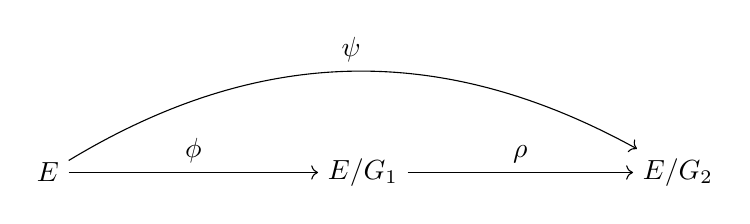
\begin{tikzpicture}
        \node (E0) at (-4, 0) {$E$};
        \node (E1) at (0, 0) {$E/G_1$};
        \node (E2) at (4, 0) {$E/G_2$};

        \draw [->] (E0) -- (E1) node [midway, above] {$\phi$};
        \draw [->] (E1) -- (E2) node [midway, above] {$\rho$};
        \draw [->] (E0) to [bend left] node [midway, above] {$\psi$} (E2);
    \end{tikzpicture}
\end{center}
is commutative.
An analogous statement also holds for inseparable isogenies.
If $\mathrm{char}(k) = p$, then an inseparable isogeny $\psi: E \to E'$ always factors through the $p$-th power Frobenius $\pi: E \to E^{(p)}$ (which is of course purely inseparable), where $E^{(p)}$ is the Elliptic Curve with all coefficients of the defining equation raised to the $p$-th power.
Note that can also define operation $\cdot^{(p)}$ on isogenies, by again raising each coefficient in the defining polynomials to the $p$-th power.
This way, $\cdot^{(p)}$ becomes an endofunctor on the category of Elliptic Curves over $\bar{\F}_p$ and their isogenies.

The final notion we require in this context is the one of the dual isogeny.
Since the kernel of an isogeny $\psi: E \to E'$ is a subgroup of size $\deg_s(\psi)$, we see that it is contained in $E[\deg(\psi)] = \ker[\deg(\psi)]$.
Now the previous correspondence shows that $\psi$ factors through through the multiplication map $[\deg(\psi)]$, via an isogeny $\hat{\psi}$
\begin{center}
    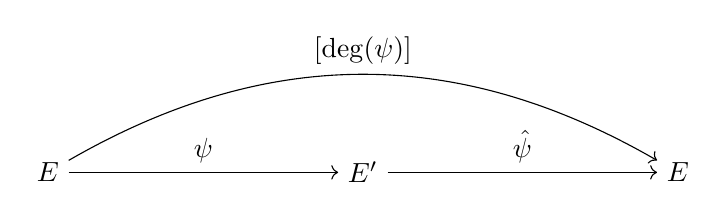
\begin{tikzpicture}
        \node (E0) at (-4, 0) {$E$};
        \node (E1) at (0, 0) {$E'$};
        \node (E2) at (4, 0) {$E$};

        \draw [->] (E0) -- (E1) node [midway, above] {$\psi$};
        \draw [->] (E1) -- (E2) node [midway, above] {$\hat{\psi}$};
        \draw [->] (E0) to [bend left] node [midway, above] {$[\deg(\psi)]$} (E2);
    \end{tikzpicture}
\end{center}
The isogeny $\hat{\psi}: E' \to E$ has then the same degree as $\psi$, and is called the \emph{dual isogeny} of $\psi$.

Interestingly, the dual isogeny behaves like an adjoint w.r.t. the Weil pairing, i.e.
\begin{equation*}
    e_m(S, \phi(T)) = e_m(\hat{\phi}(S), T)
\end{equation*}
for an isogeny $\phi: E \to E'$ and the $m$-th Weil pairing $e_m$ of $E$ resp. $E'$ (see \cite[Prop.~III.8.2]{arithmetic_elliptic_curves}).

\section{The endomorphism ring}
For an Elliptic Curve $E$, we write from now on $\End(E)$ for the set of isogenies $E \to E$.
Via composition and pointwise addition, this becomes a (possibly noncommutative) unital ring.
The existence of the multiplication-by-$m$ isogeny implies that there is a ring homomorphism
\begin{equation*}
    \Z \to \End(E)
\end{equation*}
As it turns out, this is always injective \cite[Prop.~III.4.2]{arithmetic_elliptic_curves}, hence the endomorphism ring has characteristic 0.
Much more is known about the endomorphism ring, though.
In particular, there is the following theorem
\begin{theorem}
    Let $E$ be an Elliptic Curve over $k$. Then $\End(E)$ is one of the following
    \begin{itemize}
        \item The ring of integers $\Z$.
        \item An order in a quadratic imaginary number field.
        \item An order in the quaternion algebra ramified exactly at $p$ and $\infty$, where $p = \mathrm{char}(k)$.
    \end{itemize}
    If $\mathrm{char}(k) = 0$, only the first two are possible.
    Similarly, if $\mathrm{char}(k) \neq 0$, only the last two are possible. 
\end{theorem}
For a proof, see e.g. \cite[Corollary~III.9.4]{arithmetic_elliptic_curves}.

If $\mathrm{char}(k) \subseteq \bar{\F}_p$, we call the curve $E$ \emph{ordinary} in the second case and \emph{supersingular} in the third case.
There are some other fundamental differences between those two types, as displayed in the following table.
Denote by $\pi_E$ the $q$-th power Frobenius, where $E$ is defined over $\F_q$.
\begin{center}
    \begin{tabular}{c | c}
        ordinary & supersingular \\
        \hline
        $[p]$ has separability degree $p$ & $[p]$ is totally inseparable \\
        $E[p] \cong \Z/p\Z$ & $E[p] = \{ \IdPoint \}$ \\
        $\End(E)$ is commutative & $\End(E)$ is not commutative \\
        $\mathrm{Tr}(\pi_E) \not\equiv 0 \mod p$ & $\mathrm{Tr}(\pi_E) \equiv 0 \mod p$ \\
        $\hat{\pi}_E$ separable & $\hat{\pi}_E$ totally inseparable \\
        $p \notdivides d(\End(E))$ and $p \notdivides d(\Z[\pi_E])$ & $p \divides d(\Z[\pi_E])$
    \end{tabular}
\end{center}
Note that the trace
\footnote{By trace, we mean either the trace in the quadratic imaginary number field, or the reduced trace in the quaternion algebra. In particular, if $\pi_E = \pm p$ (the supersingular setting with $E/\F_{p^2}$), we have $\mathrm{Tr}(\pi_E) = \pm 2p$.}
of the Frobenius endomorphism $\mathrm{Tr}(\pi_E)$ is of some importance, as (in the ordinary case) it determines the quadratic imaginary number field that contains $\End(E)$.
Furthermore, there is the relationship
\begin{equation*}
    \mathrm{Tr}(\pi_E) = q + 1 - \#E(\F_q)
\end{equation*}
There is also the famous theorem by Hasse \cite[Thm V.1.1]{arithmetic_elliptic_curves} which states that
\begin{equation*}
    |\#E(\F_q) - q - 1| \leq 2\sqrt{q}
\end{equation*}
In particular, this implies that $|\mathrm{Tr}(\pi_E)| \leq 2\sqrt{q}$.
Furthermore, if $E/\F_q$ is ordinary, the discriminant of the order $\End(E)$ divides the discriminant $d(\Z[\pi_E])$, as $\Z[\pi_E] \subseteq \End(E)$.
As $d(\Z[\pi_E]) = \mathrm{Tr}(\pi_E)^2 - 4q$, we see that $-4q < d(\End(E)) < 0$ in this case.

Finally, note that in a supersingular Elliptic Curve, we always have $[p] = \epsilon \pi^2$, where now $\pi: E \to E^{(p)}$ the the $p$-th power Frobenius and $\epsilon$ is an automorphisms of $E$.
However, too hard to show \cite[Thm~III.10.1]{arithmetic_elliptic_curves} that
\begin{equation*}
    \#\mathrm{Aut}(E) = \begin{cases}
        2 & \text{if $j(E) \neq 0, 1728$} \\
        4 & \text{if $j(E) = 1728$} \\
        6 & \text{if $j(E) = 0$}
    \end{cases}
\end{equation*}
in the case $\mathrm{char}(k) \neq 2, 3$.
Thus we see that either $j(E) \in \{ 0, 1728 \}$ or $[p] = \pm\pi^2$, and so in both cases that $j(E) \in \F_{p^2}$.
In other words, every supersingular curve is isomorphic to a curve over $\F_{p^2}$.

\chapter{Isogeny graphs}


In cryptography, we are of course not just interested in abstract structure of Elliptic Curves and isogenies, but also in computing it.
There are for example nice ways to compute the curve $E$ and the isogeny $E \to E/G$ for a finite subgroup $G \leq E$ in time polynomial in $\#G$.
However, in the general case, there is no way how one can represent or compute an isogeny of exponentially large degree.
This is where we can do cryptography, since for smooth-degree isogenies $\psi$, we can factor them into a sequence of small degree isogenies, and evaluate them one after the other.
However, if this factorization is not known, it seems very hard to evaluate the isogeny.

The underlying structure of this approach (and others) can now be captured by the $l$-isogeny graph $\Gamma_l(\F_q)$, for a prime $l \neq p$.
\begin{definition}
    Denote by $\Gamma_l(\F_q)$ the graph whose vertices are isomorphism classes of Elliptic Curves over $\F_q$, and the edges are the degree $l$ isogenies between them (with multiplicity).
\end{definition}
Since there is never an isogeny between ordinary and supersingular curves, each connected component of $\Gamma_l(\F_q)$ contains either only ordinary or supersingular curves.
Hence, we will call them ordinary and supersingular connected components, respectively.
Furthermore, the existence of the dual isogeny shows that this graph is undirected, and we know that it is $(l + 1)$-regular (if $l \perp p$), since there are exactly $l + 1$ subgroups of order $l$ in $E[l] \cong (\Z/l\Z)^2$.

Note that when doing computations with this graph, we identify each vertex with the j-invariant of the corresponding curves.
This makes it easy to work with isomorphism classes of Elliptic Curves.
Furthermore, we observe that $\Gamma_l(\F_q)$ has exactly $q$ vertices, since there are that many j-invariants $j \in \F_q$.

\section{The ordinary case}
We begin by analysing the structure of the ordinary part of $\Gamma_l(\F_q)$, which (as we will see), is quite different from the supersingular part.
There is a very powerful description of this graph in terms of the endomorphism rings of the ordinary curves.
Since these are (usually non-maximal) orders in quadratic imaginary number fields, whose theory is somewhat more complicated than the one of maximal orders (which are Dedekind domains), we first study them a little.

\subsection{Imaginary quadratic orders}
For this part, let $\O$ be an order in an imaginary quadratic number field $K$.
What we will mainly do in this section is to show that ideal $\a \leq \O$ with norm $\Norm(\a) := [\O : \a]$ coprime to the index $[\O_K : \O]$ behave ``nicely'', i.e. similar to ideals in a Dedekind domain.
Furthermore, we will study the structure of the class group of $\O$.
First, we state a version of the chinese remainder theorem.
\begin{lemma}
    Let $\a$ be a nonzero ideal of $\O$. Then
    \begin{equation*}
        \O/\a \cong \bigoplus_\p \O_\p/\a\O_\p
    \end{equation*}
\end{lemma}
For a proof of this, see e.g. \cite[Prop.~I.12.3]{neukirch}.
\begin{lemma}
    Let $\p \leq \O_K$ be a prime with $\Norm(\p) \perp [\O_K : \O]$.
    Then $\p$ has a set of generators in $\O$.
\end{lemma}
\begin{proof}
    Suppose $\p$ is a prime over $p$, and let $\O = \Z[\phi]$.
    We use the decomposition law in Dedekind ring extensions.
    Since $\Norm(\p) \perp [\O_K : \O]$ are coprime, we can apply it with a generator $\phi$ of $\O$.

    If $\mathrm{MiPo}(\phi) = f(X)g(X) \mod p$ splits, then have
    \begin{equation*}
        p\O_K = (p, f(\phi))(p, g(\phi))
    \end{equation*}
    and so the prime ideals over $p$ are $(p, f(\phi))$ and $(p, g(\phi))$.
    If $\mathrm{MiPo}(\phi) \mod p$ is irreducible, then have that $p\O_K$ is prime and thus the only prime ideal over $p$.
    Hence, all prime ideals over $p$ (including $\p$) have a set of generators in $\O$.
\end{proof}
\begin{corollary}
    \label{prop:generators_in_order}
    Let $\a \leq \O_K$ be an ideal with $\Norm(\a) \perp [\O_K : \O]$. Then $\a$ has a set of generators in $\O$.
\end{corollary}
\begin{prop}
    \label{prop:prime_coprime_localization_same}
    Let $\p \leq \O$ be a prime ideal with $\Norm(\p) \perp [\O_K : \O]$ and $\p' = \p\O_K$.
    Then $\O_\p = (\O_K)_{\p'}$.
\end{prop}
\begin{proof}
    We have $\O_K = \Z[\alpha]$ and $\O = \Z[f\alpha]$ where $f = [\O_K : \O]$.
    Thus $f \notin \p$ and so $f \in \O_\p^*$.
    Therefore $\O_K \subseteq \O_\p$ and thus $(\O_K)_{\p'} \subseteq \O_\p$.
\end{proof}
This already gives a somewhat nice description of most ideals of the order $\O$.
\begin{prop}
    \label{prop:coprime_ideals_order}
    Let $\mathfrak{I}_f(\O)$ resp. $\mathfrak{I}_f(\O_K)$ denote the monoid of invertible integral ideals of norm $\perp f := [\O_K : \O]$.
    Then
    \begin{align*}
        \mathfrak{I}_f(\O) \to \mathfrak{I}_f(\O_K), \quad \a \mapsto \a\O_K
    \end{align*}
    is a monoid isomorphism with inverse
    \begin{equation*}
        \mathfrak{I}_f(\O_K) \to \mathfrak{I}_f(\O), \quad \a \mapsto \a \cap \O
    \end{equation*}
\end{prop}
\begin{proof}
    Clearly, this is a well-defined monoid homomorphism.
    Hence, we have to show that it is bijective.

    By Corollary~\ref{prop:generators_in_order}, we know that any $\a \leq \O_K$ with $\Norm(\a) \perp [\O_K : \O]$ has generators in $\O$, thus $(\a \cap \O)\O_K = \a$.
    This shows that $\a \cap \O$ is a preimage of $\a$, and so the map is surjective. 

    Assume now $\a, \b \leq \O$ with $\a\O_K = \b\O_K$ and $\Norm(\a), \Norm(\b) \perp f$.
    We show that $\a_\p = \b_\p$ for all primes $\p \leq \O$.
    Note that if $\Norm(\p) \not\perp f$, this holds trivially, as $\a_\p = \O_\p = \b_\p$.
    Otherwise, note that
    \begin{equation*}
        \a_\p = \a_\p \O_\p = \a (\O_K)_\p = \a\O_K(\O_K)_\p = \b\O_K(\O_K)_\p = \b_\p (\O_K)_\p = \b_\p
    \end{equation*}
    as $\O_\p = (\O_K)_\p$.
    This shows that $\a_\p = \b_\p$ at all primes, so $\a = \b$ and our map is injective.
    Furthermore, since $(\a \cap \O)\O_K = \a$, we see that it has the inverse
    \begin{equation*}
        \mathfrak{I}_f(\O_K) \to \mathfrak{I}_f(\O), \quad \a \mapsto \a \cap \O
    \end{equation*}
    which must then be well-defined.
\end{proof}
Furthermore, we are really interested in the class group of $\O$, which is now the quotient of only the invertible ideals of $\O$ modulo the principal ideals.
The following statements are special cases of the general theory in \cite[Chapter I.§12]{neukirch}.
\begin{lemma}
    \label{prop:invertible_ideal_characterization}
    Write $\mathfrak{I}(\O)$ for the group of invertible fractional ideals in $\O$.
    Then there exists an isomorphism
    \begin{equation*}
        \iota: \bigoplus_\p K^*/\O_\p^* \to \mathfrak{I}(\O)
    \end{equation*}
    with $\iota(a)\O_\p = (a_\p)$ for all prime ideals $\p \leq \O$ and $a = (a_\p)_\p$.
\end{lemma}
\begin{proof}
    Again, this is a special case of \cite[Prop.~I.12.9]{neukirch}.

    First, we show that for an invertible ideal $\a = (a_1, ..., a_n)$ have that $\a\O_\p$ is principal.
    By assumption, have $\a\b = (1)$ with $\b = (b_1, ..., b_m)$ and so have $1 = \sum a_i b_i c_i$ with $c_i \in \O_\p$.
    Clearly, $1 \notin \p\O_\p$ and thus one $a_i b_i c_i \notin \p\O_\p$, so $a_i b_i c_i \in \O_\p^*$ is a unit.
    Therefore, we find that $\a\O_\p = a_i\O_\p$, because for all $x \in \a\O_\p$, have then $x b_i c_i \in \a\b = \O_\p$, so
    \begin{equation*}
        x = a_i \underbrace{x b_i c_i}_{\in \O_\p} \in a_i \O_\p
    \end{equation*}
    Now we can see that there is a well-defined homomorphism
    \begin{equation*}
        \iota^{-1}: \mathfrak{I}(\O) \to \bigoplus_\p K^*/\O_\p^*
    \end{equation*}
    that maps an ideal $\a$ to the class of generators of $\a\O_\p$.
    
    Clearly, it is injective, since if $\a\O_\p \neq \b\O_\p$ for any prime $\p$, then $\a \neq \b$.

    It is thus left to show that $\iota^{-1}$ is also surjective.
    The following proof is taken with some modifications from \cite[Prop.~I.12.2]{neukirch}.

    Assume $(a_\p)_\p \in \bigoplus_\p K^*/\O_\p^*$.
    Then set $\a := \bigcap_\p a_\p \O_\p$.
    Clearly we have $\a\O_\p \subseteq a_\p\O_\p$, so it is left to show the inclusion $\supseteq$.

    First of all, all except finitely many $a_\q$ are in $\O_\q^*$, hence we can assume that those are $a_\q = 1$.
    Let $c \in \O$ with $ca_\q/a_\p \in \O$ for all $\q$ such that $a_\q \neq 1$.
    Now the chinese remainder theorem gives us $b \in \O$ such that
    \begin{equation*}
        b \equiv c \mod \p \quad \text{and} \quad b \equiv ca_q/a_\p \mod \q^k \quad \text{for $\q \neq \p$ with $a_\q \neq 1$}
    \end{equation*}
    where $k \geq 1$ is an integer such that $a_q \in \q^k\O_k$.

    This $b$ is unique modulo $\bigcap_{a_\q \neq 1} \q^k$, and in particular, we can choose it such that $ba_\p/c \in \O$.
    Now we have $b/c \in \O_\p^*$.
    Furthermore, $a_\p b/c \in \a$, since
    \begin{itemize}
        \item $b/c \in \O_\p^* \subseteq \O_\p$, so $a_\p b/c \in a_\p\O_\p$.
        \item $b \equiv ca_q/a_\p \mod \q^k$, so $a_\p b/c \equiv a_\q \mod \q^k\O_\q$, which implies $a_\p b/c \in a_\q\O_\q$ for $\q \neq \p$ with $a_\q \neq 1$.
        \item $ba_\p/c \in \O$, so $ba_\p/c \in a_\q\O_\q$ whenever $a_\q = 1$.
    \end{itemize}
    Since $b/c \in \O_\p^*$, we now find $a_\p \in \a\O_\p^*$ and the claim follows.
\end{proof}
This lemma is a very useful characterization of invertible ideals.
We are now ready for our first description of $\Cl(\O)$.
\begin{lemma}
    Let $f = [\O_K : \O]$ and assume that $\O_K^* = \{ \pm 1 \}$.
    There is an exact sequence
    \begin{equation*}
        1 \ \to \ \bigoplus_\p R_\p^*/\O_\p^* \ \to \ \Cl(\O) \ \to \ \Cl(\O_K) \ \to \ 1
    \end{equation*}
    where $\Cl(\O)$ is the ideal class group of $\O$, i.e. the group of invertible, fractional ideals modulo principal ideals and $R_\p$ is the localization of $\O_K$ at the multiplicative set $\O \setminus \p$.
\end{lemma}
\begin{proof}
    This proof is taken with some modifications from \cite[Prop.~I.12.11]{neukirch}.

    First, we show that every ideal class $[\a] \in \Cl(\O_K)$ has an integral representative of norm coprime to $f$.
    Let $m \divides \Norm(\a)$ be maximal such that $m \divides f^e$ for some $e$.
    Then there is an element $\alpha \in m\a^{-1}$, and we see that $\Norm(\alpha^{-1}\a) \divides \Norm(\a)/m$, thus is coprime to $f$.
    Furthermore, $\alpha \in \a^{-1}$, so $\alpha^{-1}\a$ is integral.
    This shows our claim, and so by Corollary~\ref{prop:generators_in_order} that the natural map
    \begin{equation*}
        \Cl(\O) \to \Cl(\O_K), \quad [\a] \to [\a\O_K]
    \end{equation*}
    is surjective.

    Next, note that the isomorphism $\iota: \mathfrak{I}(\O) \to \bigoplus_\p K^*/\O_\p^*$ induces a map
    \begin{equation*}
        \bigoplus_\p R_\p^*/\O_\p^* \to \Cl(\O)
    \end{equation*}
    where $R_\p$ is the localization of $\O_K$ at the multiplicative subset $\O \setminus \p$.

    It is injective, as for an element $a = (a_\p)_\p$ in the kernel, have that $\iota(a) = (\alpha)$.
    However, then $(a_\p) = (\alpha)$ in $\O_\p$.
    Hence, $\a_\p = \alpha\epsilon$ for $\epsilon \in \O_\p^*$ and we can assume that the representatives $a_\p \in R_\p^*$ are chosen such that $a_\p = \alpha$.
    This implies that $\alpha \in \bigcap_\p R_\p^* = \O_K^*$, and by the assumption $\O_K^* = \{ \pm 1 \}$, have then $\alpha = \pm 1$.
    The claim follows.

    Now it is only left to show that the sequence is exact at $\Cl(\O)$.

    For $a = (a_\p)_\p \in \bigoplus_\p R_\p^*/\O_\p^*$, we know that
    \begin{equation*}
        \iota(a)R_\p = \iota(a)\O_\p R_\p = a_\p R_\p = R_\p
    \end{equation*}
    and so $\mathrm{im}(f) \subseteq \ker(g)$.
    Now we show the converse.

    Let $\a \leq \O$ be integral and invertible with $\a\O_K = (\alpha)$.
    Since $[\frac 1 \alpha \a] = [\a]$ are in the same ideal class, we can assume wlog that $\alpha = 1$.

    Let $a = (a_\p)_\p = \iota^{-1}(\a)$.
    Then
    \begin{equation*}
        a_\p R_\p = a_\p\O_\p R_\p = \iota(a)R_\p = \a R_\p = \alpha R_\p = R_\p
    \end{equation*}
    This clearly implies that $a_\p \in R_\p^*$ and so $\a \in \mathrm{im}(f)$.
\end{proof}
The expression $\bigoplus_\p R_\p^*/\O_\p^*$ is still somewhat unwieldy, but fortunately, it has the following nice form.
\begin{lemma}
    We have
    \begin{equation*}
        (\O_K/f\O_K)^*/(\O/f\O_K)^* \cong \bigoplus_\p R_\p^*/\O_\p^*
    \end{equation*}
    Note that $f\O_K \subseteq \O$ is the largest ideal of $\O_K$ contained in $\O$, and thus an ideal of $\O$ as well.
\end{lemma}
\begin{proof}
    First, note that if $\Norm(\p) \perp f$, we know that $R_\p = (\O_K)_{\p\O_K}$ and so by Prop.~\ref{prop:prime_coprime_localization_same} that $R_\p^*/\O_\p^*$ is trivial.
    
    Note that for each prime $\p \leq \O$ containing $f\O_K$ have a finite, positive number of primes $\q \leq \O_K$ with $\q \cap \O = \p$.
    There is at least one, as $\p\O_K$ is contained in a prime, and the number is finite, as $f\O_K$ factors into finitely many primes in the Dedekind ring $\O_K$.
    Hence, we have by the chinese remainder theorem
    \begin{equation*}
        (\O/f\O_K)^* \cong \bigoplus_{\p \supseteq f\O_K} (\O_\p/f\O_K\O_\p)^* \cong \bigoplus_{\p \supseteq f\O_K} (\O_\p/f\O_K\O_\p)^* = \bigoplus_{\p \supseteq f\O_K} (\O_\p/fR_\p)^*
    \end{equation*}
    Furthermore, we have
    \begin{equation*}
        (\O_K/f\O_K)^* \cong \bigoplus_{\q \supseteq f\O_K} ((\O_K)_\q/f(\O_K)_\q)^* \cong \bigoplus_{\p \supseteq f\O_K} \bigoplus_{\q \supseteq \p\O_K} ((\O_K)_\q/f(\O_K)_\q)^*
    \end{equation*}
    We claim that
    \begin{equation*}
        R_\p/fR_\p \cong \bigoplus_{\q \supseteq \p\O_K} (R_\p)_\q/f(R_\p)_\q = \bigoplus_{\q \supseteq \p\O_K} (\O_K)_\q/f(\O_K)_\q
    \end{equation*}
    This isomorphism follows from the chinese remainder theorem and the fact that the prime ideals $\q$ over $\p\O_K$ give all prime ideals of $R_\p$.
    
    Both isomorphisms are compatible
    \footnote{Meaning the inclusion $\O/f\O_K \subseteq \O_K/f\O_K$ commutes with the natural map
    \begin{equation*}
        O/f\O_K \overset{\sim}{\to} \bigoplus_\p (\O_\p/f\O_K\O_\p) = \bigoplus_\p (\O_\p/fR_\p) \to \bigoplus_\p (R_\p/fR_\p) \overset{\sim}{\to} \O_K/f\O_K
    \end{equation*}
    }, 
    and so have
    \begin{equation*}
        (\O_K/f\O_K)^*/(\O/f\O_K)^* \cong \bigoplus_{\p \supseteq f\O_K} (R_\p/fR_\p)^*/(\O_\p/fR_\p)^*
    \end{equation*}
    Finally, observe that the map $R_\p^* \to (R_\p/fR_\p)^*/(\O_\p/fR_\p)^*$ has kernel $\O_\p^*$.
    It also is surjective, since for $[a] \in (R_\p/fR_\p)^*$ there is $b \in R_\p$ with $ab \in 1 + fR_\p$ and thus $ab \equiv 1 \mod \p R_\p$ (because we only consider $\p$ with $f \in \p$).
    In particular, $a \notin \q$ for all primes $\q$ of $R_\p$ (these are all over $\p R_\p$), and so $a \in R_\p^*$.
\end{proof}
\begin{corollary}
    \label{prop:class_group_order}
    Suppose $\O_K = \{ \pm 1 \}$. Then there is an exact sequence
    \begin{equation*}
        1 \ \to \ (\O_K/f\O_K)^*/(\O/f\O_K)^* \ \to \ \Cl(\O) \ \to \ \Cl(\O_K) \ \to \ 1
    \end{equation*}
\end{corollary}
The condition $\O_K = \{ \pm 1 \}$ is very weak, as there are only two quadratic imaginary number fields such that the ring of integers has more units, namely $K = \Q[\sqrt{-3}]$ and $K = \Q[\sqrt{-1}]$.
These correspond to the Elliptic Curves with j-invariants $0$ and $1728$ (if they are ordinary), and need a special treatment in many cases anyway.
In \cite{neukirch}, there is also a more general version of this statement without this assumption.

\subsection{The class group action}
Now we can come back to the study of Elliptic Curves and their isogeny graphs.
The class group action which we will define in the following is the most important tool when working with isogeny graphs of ordinary curves.
Because of this, it is mentioned in more or less all the literature dealing with the topic.
For me, it was thus quite surprising that I could nowhere find a precise and relatively elementary proof for the statement in the case of finite fields.

Most sources cite \cite[Thm~4.5]{class_group_action_waterhouse}, however the statement there is not as explicit as one might wish, and the proof is done in the much more general theory of abelian schemes.
Apart from that, there are many references to the corresponding statement for curves over $\C$, but these ignore some of the subtleties introduced by non-separable isogenies. 
Therefore, we now present a relatively simple proof of the class group action for ordinary curves defined over a finite field and explicitly handle the non-separable case.

For the whole section, let $E$ and $E'$ be Elliptic Curves defined over a finite field $k = \F_q$ with characteristic $p$.
We write $\pi_E$ for the $q$-th power Frobenius endomorphism of $E$.
\begin{definition}
    For an integral ideal $\a \leq \End(E)$ of an ordinary Elliptic Curve $E$, define the $\a$-torsion
    \begin{equation*}
        E[\a] := \bigcap_{\alpha \in \a} \ker(\alpha)
    \end{equation*}
\end{definition}
From now on, we will often compare endomorphism rings of isogeneous curves.
To do so, we embed those rings into an imaginary quadratic number field $K$.
However, the field $K$ and its orders can have nontrivial automorphisms, which means the embedding $\End(E) \to K$ cannot be unique.
Fortunately, we can choose a system of embeddings $\End(E) \to K$ jointly for all curves $E$ in a canonical way as follows.
\begin{lemma}
    Let $\phi: E \to E'$ be an isogeny.
    Then there is an isomorphism
    \begin{equation*}
        \Phi: \End(E) \otimes \Q \to \End(E') \otimes \Q, \quad \tau \mapsto \frac 1 {\deg(\phi)} \phi \circ \tau \circ \hat{\phi}
    \end{equation*}
    Furthermore, if we assume $E$ to be ordinary, then this is canonical in the sense that for any other isogeny $\psi: E \to E'$ have $\Phi = \Psi$.
\end{lemma}
\begin{proof}
    It is clear that this is a morphism of ring, and its inverse is given by $\hat{\Phi}$ induced by the dual isogeny $\hat{\phi}$.
    
    So it remains to show the last part.
    Let $\phi$ and $\psi$ be two isogenies $E \to E'$.
    Then for each $\tau \in \End(E)$ have
    \begin{align*}
        (\Phi \circ \hat{\Psi})(\tau) =& \frac 1 { \deg(\phi) } \phi \circ \left( \frac 1 {\deg(\psi)} \hat{\psi} \circ \tau \circ \psi \right) \\
        =& \frac 1 { \deg(\phi)\deg(\psi) } (\phi \circ \hat{\psi}) \circ \tau \circ (\psi \circ \hat{\phi}) \\
        =& \frac 1 { \deg(\phi)\deg(\psi) } (\phi \circ \hat{\psi}) \circ (\psi \circ \hat{\phi}) \circ \tau \\
        =& \frac 1 { \deg(\phi)\deg(\psi) } (\deg(\phi) \deg(\psi)) \tau = \tau
    \end{align*}
    since $(\psi \circ \hat{\phi})$ and $\tau$ are elements of $\End(E)$, hence commute.

    Now $\hat{\Psi}$ is the inverse of $\Psi$, and the claim follows.
\end{proof}
In other words, we choose an arbitrary embedding $\End(E) \to K$ for one ordinary curve $E$, and then choose all further embeddings $\End(E') \to K$ for isogeneous curves $E'$ as
\begin{equation*}
    \End(E') \to \End(E') \otimes \Q \ \overset{\Phi}{\longrightarrow} \ \End(E) \otimes \Q \to K
\end{equation*}
From now on, whenever we identify $\End(E)$ with an approriate subring of $K$, this shall use that embedding.
It will already be used in the next statement, which describes the relationship of endomorphism rings of isogeneous curves more concretely.
\begin{prop}
    Let $\phi: E \to E'$ be an isogeny of prime degree $p$ between ordinary Elliptic Curves.
    Then (after embedding $\End(E')$ via $\Phi$ and $\End(E)$ into $\End(E) \otimes \Q$) exactly one of the following is the case.
    \begin{itemize}
        \item $\End(E) = \End(E')$ and we call $\phi$ \emph{horizontal}.
        \item $\End(E) \subseteq \End(E')$ with $[\End(E') : \End(E)] = p$. We call $\phi$ \emph{ascending}.
        \item $\End(E) \supseteq \End(E')$ with $[\End(E) : \End(E')] = p$. We call $\phi$ \emph{descending}.
    \end{itemize}
\end{prop}
\begin{proof}
    Note that the map
    \begin{equation*}
        l\Phi: \End(E) \to \End(E'), \quad \tau \mapsto \phi \circ \tau \circ \hat{\phi}
    \end{equation*}
    yields endomorphisms of $\End(E')$, and so we have $l\End(E) \subseteq \End(E')$.
    Similarly, find $l\End(E') \subseteq \End(E)$.

    Now let $\alpha$ be a generator of the maximal order in $K = \End(E) \otimes \Q$.
    Then each order of $K$ is of the form $\Z + f\alpha\Z$, and so
    \begin{equation*}
        \End(E) = \Z \oplus f_1\alpha\Z, \quad \End(E') \Z \oplus f_2\alpha\Z
    \end{equation*}
    However, this implies that $f_1 \divides lf_2$ and $f_2 \divides lf_1$, so $f_1 \divides l f_2 \divides l^2 f_1$.
    Since $l$ is prime, we find $f_2 \in \{ f_1/l, f_1, l f_1 \}$ and the claim follows.
\end{proof}
Furthermore, we will sometimes talk about horizontal or vertical isogenies \emph{at a prime $l$}, which is defined by the next proposition.
The advantage is that this is defined for all isogenies, not just those of prime degree.
\begin{prop}
    Similarly, let $\phi: E \to E'$ be an isogeny of any degree $n$.
    Further, let $l$ be a prime.
    Then (after embedding $\End(E') \otimes \Z_{(l)}$ via $\Phi$ and $\End(E) \otimes \Z_{(l)}$ into $\End(E) \otimes \Q$) exactly one of the following is the case.
    \begin{itemize}
        \item $\End(E) \otimes \Z_{(l)} = \End(E') \otimes \Z_{(l)}$ and we call $\phi$ \emph{horizontal at $l$}.
        \item $\End(E) \otimes \Z_{(l)} \subseteq \End(E') \otimes \Z_{(l)}$ with $[\End(E') \otimes \Z_{(l)} : \End(E) \otimes \Z_{(l)}] = l^r$ for $r > 0$. We call $\phi$ \emph{ascending at $l$}.
        \item $\End(E) \otimes \Z_{(l)} \supseteq \End(E') \otimes \Z_{(l)}$ with $[\End(E) \otimes \Z_{(l)} : \End(E') \otimes \Z_{(l)}] = p$ for $r > 0$. We call $\phi$ \emph{descending at $l$}.
    \end{itemize}
\end{prop}
\begin{proof}
    Exactly as the previous proof.
\end{proof}
Now we can make a step towards the class group action and present how we assign isogenies to (integral, invertible) ideals of the endomorphism ring.
\begin{definition}
    For an ordinary Elliptic Curve $E$ and an integral, invertible ideal
    \footnote{By Prop.~\ref{prop:coprime_ideals_order}, this representation of an ideal $\a$ is well-defined and unique, as $\Norm((p, \pi)) = p \notdivides [\O_{\End(E) \otimes \Q} : \End(E)] \divides d(\End(E))$.}
    $\a = \b(p, \pi_E)^r \leq \End(E)$ with $\b \perp (p, \pi_E)$ define the isogeny
    \begin{equation*}
        \phi_{E, \a}: E \ \longrightarrow \ E/E[\b] \ \overset{\pi_r}{\longrightarrow} \ E_\a := (E/E[\b])^{(p^r)}
    \end{equation*}
    where $E \to E/E[\b]$ is the unique separable isogeny with kernel $E[\b]$ and $\pi_r: E/E[\b] \to (E/E[\b])^{(p^r)}$ is the $r$-th power Frobenius map.
\end{definition}
In order to define a group action later, we need to be able to chain such isogenies given by ideals.
The obvious difficulty here is that the ideals are all in the same ring, but subsequent isogenies will have different curves as domain.
Hence, we need to be able to view an ideal $\a \leq \End(E)$ as an ideal of another endomorphism ring $\End(E')$.
As it turns out, the endomorphism rings we consider are all isomorphic, and so this works out nicely. 
\begin{lemma}
    Let $E$ be an ordinary Elliptic Curve and $\a \leq \End(E)$ an integral, invertible ideal.
    Then $\End(E) \cong \End(E_\a)$.
    In particular, $\phi_{E, \a}$ is horizontal at every prime $l$.
\end{lemma}
\begin{proof}
    Let $\a = \b(p, \pi_E)^r$ with $\b \perp (p, \pi_E)$.
    We show that $\End(E) \cong \End(E/E[\b])$ and the claim follows, as for any Elliptic Curve $E$, have an isomorphism
    \begin{equation*}
        \End(E) \to \End(E^{(p)}), \quad \alpha \mapsto \alpha^{(p)}
    \end{equation*}
    It suffices to show that the separable isogeny $\phi := \phi_{E, \b}$ is horizontal at each prime $l$.

    Assume for a contradiction that $\phi$ is descending at $l$.
    In other words, there is $\tau \in \End(E)$ such that $\phi \circ \tau \circ \hat{\phi}$ is not divisible by $l$.
    Hence, $E'[l] \not\subseteq \ker(\phi \circ \tau \circ \hat{\phi})$ and there is a point $P \in E'[l]$ with $\phi(\tau(\hat{\phi}(P))) \neq \IdPoint$.
    This implies $\tau(\hat{\phi}(P)) \notin E[\a]$ and thus there is $\alpha \in \a$ with $\tau(\hat{\phi}(P)) \notin \ker(\alpha)$.
    Note that $\alpha$ factors through $\phi$ as
    \begin{center}
        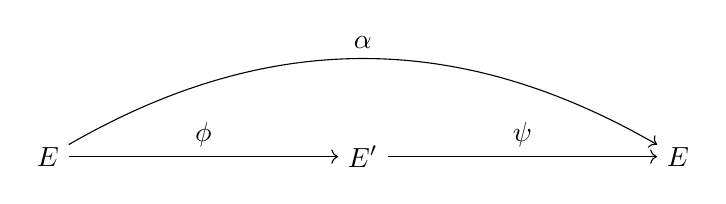
\begin{tikzpicture}
            \node (Ep) at (0, 0) {$E'$};
            \node (E1) at (-4, 0) {$E$};
            \node (E2) at (4, 0) {$E$};

            \draw [->] (E1) -- (Ep) node [midway, above] {$\phi$};
            \draw [->] (Ep) -- (E2) node [midway, above] {$\psi$};
            \draw [->] (E1) to [bend left] node [midway, above] {$\alpha$} (E2);
        \end{tikzpicture}
    \end{center}
    We assume $l \divides n$, otherwise the claim is trivial.
    However, then we have the contradiction
    \begin{align*}
        \psi((\phi \circ \tau \circ \hat{\phi})(P)) &= (\psi \circ \phi \circ \tau \circ \hat{\phi})(P) = (\alpha \circ \tau \circ \hat{\phi})(P) \\
        &= (\tau \circ \alpha \circ \hat{\phi})(P) = (\tau \circ \psi \circ [n])(P) = (\tau \circ \psi)(\IdPoint) = \IdPoint
    \end{align*}
    since $\tau \circ \alpha = \alpha \circ \tau$ ($\End(E)$ is commutative).
\end{proof}
For the next statement, we need to establish the relationship between separability of endomorphisms and properties of the endomorphism ring.
\begin{lemma}
    \label{prop:inseparable_iff_frobenius_ideal}
    Let $E$ be an ordinary curve and $\alpha \in \End(E)$.
    Then $\alpha$ inseparable if and only if $\alpha \in (p, \pi_E)$.
\end{lemma}
\begin{proof}
    First, consider
    \begin{equation*}
        \b := \{ \beta \in \End(E) \ | \ \text{$\beta$ inseparable} \}
    \end{equation*}
    This is an ideal, as for two inseparable $\beta_1, \beta_2 \in \End(E)$ have that they factor as
    \begin{center}
        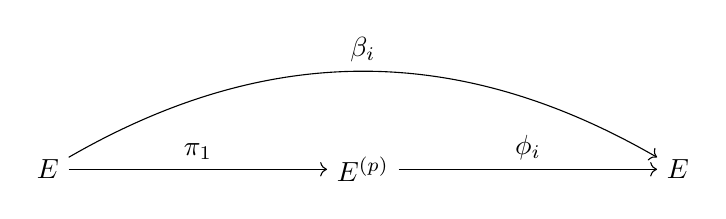
\begin{tikzpicture}
            \node (Ep) at (0, 0) {$E^{(p)}$};
            \node (E1) at (-4, 0) {$E$};
            \node (E2) at (4, 0) {$E$};

            \draw [->] (E1) -- (Ep) node [midway, above] {$\pi_1$};
            \draw [->] (Ep) -- (E2) node [midway, above] {$\phi_i$};
            \draw [->] (E1) to [bend left] node [midway, above] {$\beta_i$} (E2);
        \end{tikzpicture}
    \end{center}
    with the $p$-th power Frobenius $\pi_1: E \to E^{(p)}$.
    Now $\beta_1 + \beta_2 = (\phi_1 + \phi_2) \circ \pi_1$ is inseparable, and clearly $\beta \gamma$ is inseparable for $\beta \in \b$ and $\gamma \in \End(E)$ (just compare separability degrees).

    Furthermore, $p$ and $\pi_E$ are inseparable, so $(p, \pi) \subseteq \b$.
    Note that in the imaginary quadratic order $\End(E)$, every prime ideal is maximal.
    Since $\Norm((p, \pi)) = p \perp d(\End(E))$, Prop.~\ref{prop:coprime_ideals_order} shows that $(p, \pi_E)$ is prime, and thus $(p, \pi_E) = \b$ (clearly, $\b \neq \End(E)$).
\end{proof}
Note now that for an isogeny $\phi: E \to E'$, have
\begin{equation*}
    \phi \circ \hat{\phi} \circ \Phi(\pi_E) = \frac {\deg(\phi)} {\deg(\phi)} \phi \circ \pi_E \circ \hat{\phi}
\end{equation*}
Comparing inseparability degrees, it follows that $\Phi(\pi_E)$ is totally inseparable as endomorphism on $E'$.
Hence, $E'$ is isomorphic to a curve such that $\Phi(\pi_E)$ becomes the Frobenius endomorphism of that curve.
Since we only work with isomorphism classes, we assume from now on that $\Phi(\pi_E)$ is the Frobenius of $E'$.

Now we can prove that ideal multiplication is compatible with chaining of isogenies.
Note that the condition $p \notdivides d(\O)$ is just equivalent to all curves $E$ with $\End(E) \cong \O$ being ordinary.
\begin{lemma}
    Let $\O$ be a quadratic imaginary order with $p \notdivides d(\O)$ and two integral, invertible ideals $\a, \b \leq \O$.
    Let further $E$ be an Elliptic Curve with $\End(E) \cong \O$.
    Identifying $\End(E_\a)$ with $\O$ by the canonical isomorphism $\Phi_{E, \a}: \End(E) \overset{\sim}{\longrightarrow} \End(E_\a)$, we have
    \begin{equation*}
        E_{\a\b} \cong (E_\a)_\b \quad \text{and} \quad \phi_{E, \a\b} = \phi_{E_\a, \b} \circ \phi_{E, \a}
    \end{equation*}
\end{lemma}
\begin{proof}
    Write $\pi \in \O$ for the unique element of $\O$ that maps to the Frobenius of $E$ under the maps $\O \overset{\sim}{\longrightarrow} \End(E)$ for all $E$ with $\End(E) \cong \O$.
    
    We have $\a = \tilde{\a} (p, \pi)^r$ and $\b = \tilde{\b} (p, \pi)^s$ with $\tilde{\a}, \tilde{\b} \perp (p, \pi)$.
    It is now the case that
    \begin{equation*}
        \phi_{E, \a\b} = \phi_{E, \tilde{\a} \tilde{\b}}^{(p^{r + s})}
    \end{equation*}
    and
    \begin{equation*}
        \phi_{E_\a, \b} \circ \phi_{E, \a} = (\phi_{E_\a, \tilde{\b}} \circ \pi_r \circ \phi_{E, \tilde{\a}})^{(p^s)} = (\phi_{E_\a, \tilde{\b}}^{(q/p^r)} \circ \phi_{E, \tilde{\a}})^{(p^{r + s})}
    \end{equation*}
    where $\pi_r: E_{\tilde{\a}} \to E_{\tilde{\a}}^{(p^r)}$ is the $p^r$-th power Frobenius and we assume that $\phi_{E_\a, \tilde{\b}}$ is defined over $\F_q$.
    Note that $\phi_{E_\a, \tilde{\b}}$ is the separable isogeny with kernel $E_\a[\tilde{\b}]$ and thus $\phi_{E_\a, \tilde{\b}}^{(q/p^r)}$ is the separable isogeny with kernel $E_{\a}^{(q/p^r)}[\tilde{\b}] = E_{\tilde{\a}}[\tilde{\b}]$.
    In other words, find
    \begin{equation*}
        \phi_{E_\a, \tilde{\b}}^{(q/p^r)} = \phi_{E_{\tilde{\a}}, \tilde{\b}}
    \end{equation*}
    and so it suffices to show the claim in the case that $\a = \tilde{\a}$, $\b = \tilde{\b}$ are integral, invertible ideals coprime to $(p, \pi)$.
    By Lemma~\ref{prop:inseparable_iff_frobenius_ideal}, this means that the isogenies $\phi_{E, \a}$ and $\phi_{E_\a, \b}$ are separable.

    Having reduced everything to the separable case, it now suffices to show that $\ker(\phi_{E_\a, \b} \circ \phi_{E, \a}) = E[\a\b]$.
    For simplicity of notation, write $\phi = \phi_{E, \a}$ and $\psi = \phi_{E_\a, \b}$.
    Hence, we want to show that $\ker(\psi \circ \phi) = E[\a\b]$.

    The crucial point here is that our isomorphism $\End(E) \cong \End(E_\a)$ is given by $\Phi$.
    Since the identification of $\End(E)$ and $\End(E_\a)$ would hide this, we will be explicit in this part and write
    \begin{align*}
        i: \O \overset{\sim}{\longrightarrow} \End(E) \quad \text{and} \quad i': \O \overset{\sim}{\longrightarrow} \End(E')
    \end{align*}
    for the isomorphisms.
    Note that $\Phi \circ i = i'$.
    We have
    \begin{align*}
        \ker(\psi \circ \phi) =& \phi^{-1}(\ker\psi) = \phi^{-1}(E'[\mathfrak{a}]) = \phi^{-1}\Bigl( \bigcap_{\tau \in \mathfrak{a}} \ker(i'(\tau)) \Bigr) \\
        =& \bigcap_{\tau \in \mathfrak{a}} \phi^{-1}(\ker(i'(\tau))) = \bigcap_{\tau \in \mathfrak{a}} \ker(i'(\tau) \circ \phi) \overset{(*)}{=} \bigcap_{\tau \in \mathfrak{a}} \ker(\phi \circ i(\tau)) \\
        =& \bigcap_{\tau \in \mathfrak{a}} i(\tau)^{-1}(\ker\phi) = \bigcap_{\tau \in \mathfrak{a}} i(\tau)^{-1}(E[\mathfrak{b}]) = \bigcap_{\tau \in \mathfrak{a}, \ \rho \in \mathfrak{b}} i(\tau)^{-1}(\ker(i(\rho))) \\
        =& \bigcap_{\tau \in \mathfrak{a}, \ \rho \in \mathfrak{b}} \ker(\underbrace{i(\rho) \circ i(\tau)}_{\mathclap{= i(\rho\tau) \in i(\a\b)}}) = E[\mathfrak{b}\mathfrak{a}]
    \end{align*}
    The equality at $(*)$ holds, since
    \begin{equation*}
        i'(\tau) = (\Phi_* \circ i)(\tau) = \frac 1 {\deg(\phi)} \phi \circ i(\tau) \circ \hat{\phi} \qedhere
    \end{equation*}
\end{proof}
What we have so far is already enough to establish a monoid action
\begin{equation*}
    \mathfrak{I}(\O) \times \Ell(\O) \to \Ell(\O), \quad \a \mapsto E_{\a}
\end{equation*}
where $\mathfrak{I}(\O)$ stands for the monoid of integral invertible ideals of $\O$ and
\begin{equation*}
    \Ell(\O) := \{ \text{$E$ isomorphism class of Elliptic Curves over $\bar{\F}_p$} \ | \ \End(E) \cong \O \}
\end{equation*}
denote the set of isomorphism classes of Elliptic Curves with endomorphism ring $\O$.

Next, we investigate the torsion of this action, i.e. for which $\a$ we have $\a.E = E$.
\begin{lemma}
    Let $E$ be an ordinary curve and $\a, \b \leq \End(E)$ two integral, invertible ideals.
    Then $E_\a \cong E_\b$ if and only if $[\a] = [\b] \in \Cl(\End(E))$ are in the same ideal class.
\end{lemma}
\begin{proof}
    First, we show the direction $\Leftarrow$.
    By assumption, there are $\alpha, \beta \in \O$ such that $\alpha\a = \beta\b$.
    Thus $E_{\alpha\a} = E_{\beta\b}$ and it suffices to show that for any Elliptic Curve $E$ and $\alpha \in \End(E)$, have $E_{(\alpha)} \cong E$.

    Write $(\alpha) = (p, \pi)^r \a$ and assume that $E$ is defined over $\F_{p^s}$.
    Then $(\alpha)(p)^{\lceil r/s \rceil s - r} = (\pi)^{\lceil r/s \rceil}(\alpha')$ since $(p) = (p, \pi)(p, \pi - t)$ and $(p, \pi)^s = (\pi)$ by an easy computation.
    Furthermore, $\alpha' \notin (p, \pi)$.
    Now note that for any curve $E$, have $E_{(\pi)} = E^{(p^s)} \cong E$ and $E_{(p)} \cong E$, where the latter holds, since in the ordinary case, $p$ factors as
    \begin{center}
        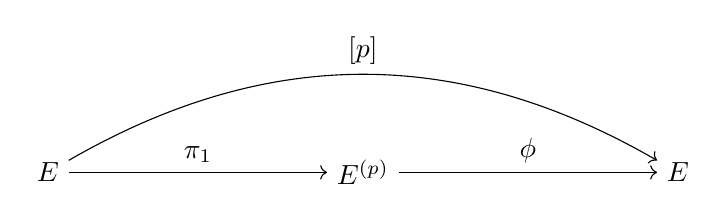
\begin{tikzpicture}
            \node (Ep) at (0, 0) {$E^{(p)}$};
            \node (E1) at (-4, 0) {$E$};
            \node (E2) at (4, 0) {$E$};

            \draw [->] (E1) -- (Ep) node [midway, above] {$\pi_1$};
            \draw [->] (Ep) -- (E2) node [midway, above] {$\phi$};
            \draw [->] (E1) to [bend left] node [midway, above] {$[p]$} (E2);
        \end{tikzpicture}
    \end{center}
    with the $p$-th power Frobenius $\pi_1$ and $\phi$ is separable with $\ker(\phi) = E[p] = \ker([p]) \cap \ker(\pi - t)$.
    Thus we see that $E_{(\alpha)} \cong E_{(\alpha')}$ and can assume wlog that $\alpha = \alpha' \notin (p, \pi)$.

    By Lemma~\ref{prop:inseparable_iff_frobenius_ideal}, we now see that $\alpha$ is separable, and so clearly $\ker(\alpha) = E[(\alpha)]$.
    Since $\alpha: E \to E$ is the separable isogeny on $E$ with kernel $E[(\alpha)]$, we see that $E_{(\alpha)} = E/E[(\alpha)] \cong E$.

    Now we consider the other direction $\Rightarrow$.
    Again, write $\a = \tilde{\a}(p, \pi)^r$ and assume that $E$ is defined over $\F_{p^s}$.
    Then we have as before that $\a (p)^{\lceil r/s \rceil s - r} = (\pi)^{\lceil r/s \rceil} \a'$ for the ideal $\a' = \tilde{\a} (p, \pi - t)^{\lceil r/s \rceil s - r}$.
    Now clearly $[\a] = [\a']$ are in the same ideal class and $\a' \perp (p, \pi)$.
    Furthermore, by the direction $\Leftarrow$, have $E_\a \cong E_{\a'}$.
    Doing the same with $\b$, we can assume wlog that $\a = \a'$ and $\b = \b'$ are ideals coprime to $(p, \pi)$.

    Therefore, the isogenies $\phi_{E, \a}$ and $\phi_{E, \b}$ are separable.
    Write $E' := E_\a = E_\b$.
    Choose $N > 0$ such that $[N]^{-1}(E[\a]) \supseteq E[\b]$.
    Now the isogeny $[N] \circ \phi_{E, \a}$ factors through $\phi_{E, \b}$, i.e. we get a commutative diagram
    \begin{center}
        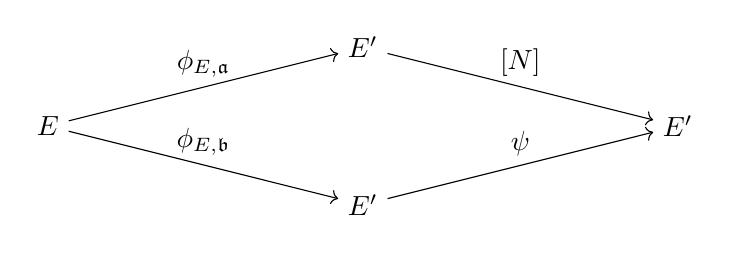
\begin{tikzpicture}
            \node (E1) at (0, 1) {$E'$};
            \node (E2) at (0, -1) {$E'$};
            \node (E0) at (-4, 0) {$E$};
            \node (E3) at (4, 0) {$E'$};

            \draw [->] (E0) -- (E1) node [midway, above] {$\phi_{E, \a}$};
            \draw [->] (E0) -- (E2) node [midway, above] {$\phi_{E, \b}$};
            \draw [->] (E1) -- (E3) node [midway, above] {$[N]$};
            \draw [->] (E2) -- (E3) node [midway, above] {$\psi$};
        \end{tikzpicture}
    \end{center}
    for some endomorphism $\psi: E' \to E'$.
    Clearly the isogenies $[N]$ and $\psi$ are given by the ideals $(N)$ resp. $(\psi)$, and so we find
    \begin{equation*}
        (N)\a = (\psi)\b
    \end{equation*}
    and the claim follows.
\end{proof}
Now we have proven almost everything we need.
The final ingredient, from which it will then follow that the class group action is transitive, is a theorem of Tate.
Since it uses much of the theory on general abelian varieties, we will present it without proof here.
For a proof, the reader is referred to the work of Tate \cite{tate}.
\begin{theorem}[Isogeny theorem]
    \label{prop:isogeny_theorem}
    Let $E$, $E'$ be Elliptic Curves defined over $\F_q$.
    Then there is an isogeny $E \to E'$ if and only if $\#E(\F_q) = \#E'(\F_q)$.
\end{theorem}
Note that this condition is also equivalent to $\End(E) \otimes \Q \cong \End(E') \otimes \Q$ or that the $q$-th power Frobenius endomorphisms have the same trace. 
\begin{theorem}
    \label{prop:class_group_action}
    Let $\O$ be an imaginary quadratic order with $p \notdivides d(\O)$.
    Then there is a free and transitive group action
    \begin{equation*}
        \Cl(\O) \times \Ell(\O) \to \Ell(\O), \quad ([\a], E) \mapsto E_\a
    \end{equation*}
    where $\a$ is an integral, invertible ideal representative of the ideal class $[\a]$.
\end{theorem}
\begin{proof}
    Well-definedness and freeness follow from all the previous lemmas.
    So it is left to derive the transitivity from Thm~\ref{prop:isogeny_theorem}.
    Let $E$ and $E'$ be curves in $\Ell(\O)$.
    Clearly, we then have $\#E(\F_q) = \#E'(\F_q)$ and so there is a separable isogeny $\phi: E \to E'$.
    Everything we have to show is that $\phi = \phi_{E, \a}$ for some ideal $\a \leq \O$.
    Note that we can multiply $\a$ by $(p)$ and divide by $\pi$, and thus achieve that $\phi$ is separable.

    Here we use the same approach as in \cite[Thm~4.5]{class_group_action_waterhouse}.
    In particular, we want to consider the problem locally at primes $l$.
    The usual way to achieve this is to consider the $l$-adic Tate module defined as the inverse limit
    \begin{equation*}
        T_lE := \lim_n E[l^n]
    \end{equation*}
    Note that this is an $\O_l := \O \otimes \Z_l$-module.
    Furthermore, the isogeny $\phi$ induces a map
    \begin{equation*}
        \phi_l: T_lE \to T_lE', \quad (P_n)_n \mapsto (\phi P_n)_n
    \end{equation*}
    By our choice of the canonical isomorphism $\End(E) \cong \O \cong \End(E')$, this becomes an $\O_l$-module homomorphism.
    Extending it linearly, we get the map
    \begin{equation*}
        \phi_l: T_lE \otimes_{\Z_l} \Q_l \to T_lE' \otimes_{\Z_l} \Q_l
    \end{equation*}
    We can now consider the $\O_l$-module $M := \phi_l^{-1}(T_lE') \subseteq T_lE \otimes_{\Z_l} \Q_l$.
    Note that this is the only time we use the assumption $\End(E) \cong \End(E')$, which yields here that $M$ is an $\O_l$-module.

    The module $M$ contains $T_lE$ and furthermore, $T_lE$ has finite index in $M$.
    Therefore $M$ is a $\O_l$-submodule of $l^{-n}T_lE$ for some $n$.

    So we see that $M$ is a free rank-1 module over $\O_l$, and hence there is an element $\alpha_l \in \O_l$ with
    \begin{equation*}
        \alpha_l M = T_lE
    \end{equation*}
    Note that we can write $\alpha_l = a \otimes l^n b$ with $a \in \O$ and $b \in \Z_l^*$.
    Then also $(al^n) M = T_lE$ and thus we can assume wlog that $\alpha_l = al^n \in \O$.

    Now it is left to establish the connection between $\ker(\phi)$ and $M$.
    This is done by the map
    \begin{equation*}
        \phi_l^{-1}(T_lE') = M \to \ker(\phi)_{(l)}, \quad \frac 1 {l^m} (P_n)_n \mapsto P_m
    \end{equation*}
    where an element of $T_lE'$ is $(P_n)_n$ with $P_n \in E[l^n]$ such that $[l]P_{n + 1} = P_n$.
    Further
    \begin{equation*}
        \ker(\phi)_{(l)} := \{ P \in \ker(\phi) \ | \ \text{$[l]^nP = \IdPoint$ for some $n \geq 0$}\}
    \end{equation*}
    is the power-of-$l$ torsion part of $\ker(\phi)$, or equivalently the localization at the prime ideal $(l)$ as $\Z$-module.

    First, note that the map is well-defined, as for an element $1/l^m (P_n)_n$ in the domain, we have by assumption
    \begin{equation*}
        \frac 1 {l^m} \phi_l((P_n)_n) = \frac 1 {l^m} (\phi(P_n))_n \in T_lE'
    \end{equation*}
    and thus $\phi(P_m) = \IdPoint$, i.e. $P_m \in \ker(\phi)$.

    Clearly, the map is also a morphism of $\O$-modules, where $\ker(\phi)_{(l)}$ becomes an $\O$-module in the obvious way.
    
    It is also surjective, since for $P \in \ker(\phi)_{(l)}$ of order $\mathrm{ord}(P) = l^m$, we can lift it to an element $(P_n)_n$ with $P_m = P$.
    Then clearly $1/l^m(P_n)_n \in M$ with image $P$.

    Finally, note that for $1/l^m(P_n)_n \in M$ have $P_m = \IdPoint$ if and only if $P_0 = ... = P_m = \IdPoint$, in which case we have that
    \begin{equation*}
        1/l^m(P_n)_n = (P_{n + m})_n \in T_lE
    \end{equation*}
    Thus the kernel of above map is $T_lE$ and we get an isomorphism of $\O$-modules
    \begin{equation*}
        \ker(\phi)_{(l)} \cong M / T_lE
    \end{equation*}

    Now let $\a \leq \O$ be the invertible ideal such that $\a\O_\l = (\alpha_l)_\l$ for every prime ideal $\l$ under a prime number $l$ (the $\alpha_l$ are the element from above with $\alpha_l M = T_lE$).
    This is possible by Lemma~\ref{prop:invertible_ideal_characterization}, as only finitely many $(\alpha_l) \neq (1)$ (namely for those $l$ with $l \divides \deg(\phi)$).

    Then for each primes $l$, we have
    \begin{equation*}
        \ker(\phi)_{(l)} = \{ P \in E_{(l)} \ | \ \alpha_l(P) = \IdPoint \} = \{ P \in E_{(l)} \ | \ \forall \alpha \in \a: \alpha(P) = \IdPoint \}
    \end{equation*}
    where again $E_{(l)}$ is the power-of-$l$ torsion part of the group $E$.
    Thus $\ker(\phi) = E[\a]$.
\end{proof}
A similar class group action exists in many other cases, since it is really founded in the theory of abelian varieties, see \cite{class_group_action_waterhouse}.
Notable examples are the CSIDH class group action for supersingular curves defined over $\F_p$ (see \cite{csidh}), its generalization to so-called oriented curves (see \cite{osidh}), and the very classical class group action of Elliptic Curves with complex multiplication (over $\C$).
More concretely, if we consider an order $\O$ in a quadratic imaginary number field and write $\Ell(\O)$ for the set of (isomorphism classes of) curves over $\C$ with endomorphism ring $\O$ (these are said to have \emph{complex multiplication}), then there is a free and transitive class group action
\begin{equation*}
    \Cl(\O) \times \Ell(\O) \to \Ell(\O), \quad ([\a], E) \to E/E[\a]
\end{equation*}
where we choose $\a$ to be an integral ideal representative of $[\a]$.
Note that for ideals $\a \perp (p, \pi)$, this is analogous to our action defined above.
However, since the Frobenius has trivial kernel, one needs some addition in the finite field case.

Note that one can still keep the simpler definition
\begin{equation*}
    \Cl(\O) \times \Ell(\O) \to \Ell(\O), \quad ([\a], E) \to E/E[\a]
\end{equation*}
also in the finite field case, if we require $\a$ to be an (integral) ideal representative of $[\a]$ that is coprime to $(p, \pi)$.
Clearly, every ideal class has such a representative, since we can multiply with the principal ideal $(p) = (p, \pi)(p, \pi - t)$ and divide out the principal ideal $(\pi) = (p, \pi)^s$.
However, some sources do not explicitly mention that $\a$ must be chosen coprime to $(p, \pi)$, which caused me some confusion at the beginning.

\subsection{Vulcanos}
Once we have the class group action, we can derive a lot of information about the structure of the ordinary part of an isogeny graph.
\begin{definition}
    For $l > 0, d \geq 0$, a graph $G$ is called \emph{$l$-vulcano of depth $d$}, if its vertices can be partitioned into a set $C$ (the ``crater'') and a set $L$ (the ``lava flows'') such that
    \begin{itemize}
        \item $G[C]$ is either a single vertex (possibly with one or two loops), two connected vertices or a cycle of at least two vertices\footnote{A cycle of two vertices shall be two vertices with a double edge.}
        \item $G[V]$ is a forest of complete $l$-ary trees of depth $d$
        \item Every vertex $v \in C$ is connected to the roots of $l + 1 - \deg_{G[C]}(v)$ trees in $G[L]$
    \end{itemize}
    In particular, every vertex in $G$ except the leaves of the trees has degree $l + 1$.
\end{definition}
The term ``vulcano'' was introduced by \cite{isogeny_vulcano}, after Kohel had mostly determined the structure of ordinary connected components in his PhD thesis.
\begin{theorem}
    \label{prop:isogeny_vulcano}
    Let $G$ be a connected component of $\Gamma_l(\F_q)$.
    Suppose that $G$ is ordinary, i.e. its vertices are (isomorphism classes of) ordinary curves.
    Then $G$ is an $l$-vulcano.
    Further, we have
    \begin{itemize}
        \item All curves on the crater have the same endomorphism ring $\O$ with $l \notdivides [\O_{\O \otimes \Q} : \O]$.
        \item All curves on the $i$-th tree level of a lava flow have the endomorphism ring $\Z + l^i\O$.
        \item The size of the crater is the order of $\l_1$ in $\Cl(\O)$, where $(l) = \l_1\l_2$ in $\O$, or 1 if $l$ is inert.
    \end{itemize} 
\end{theorem}
\begin{proof}
    This follows from the class group action and the description of the class group of quadratic imaginary orders~\ref{prop:class_group_order}.
    For the remaining details, we refer the reader to Kohel's thesis \cite[Prop.~23]{kohel}.
\end{proof}
We remark that the crater of a vulcano is a single vertex with a loop, if $(l)$ is inert in $\O$.
Furthermore, the crater consists of two connected vertices, if $(l)$ is ramified in $\O$, and is either a vertex with double loop or a cycle, if $(l)$ splits.

\section{The supersingular case}
\label{sec:supersingular_isogeny_graph}
After studying the ordinary connected components of the $l$-isogeny graph $\Gamma_l(\F_q)$, we now come to the supersingular component(s).
First, note that all supersingular j-invariants are defined over $\F_{p^2}$, and so we will assume $q = p^2$ for this section.

In the supersingular setting, the endomorphism ring is now non-commutative.
There still exists a non-commutative analogue of the class group action, but using that structure is significantly harder.
Mainly, because the theory of quaternion algebras is more complicated, and its class group structure is less studied.

Instead, there is the famous result of Pizer, which states that supersingular isogeny graphs (i.e. the supersingular part of $\Gamma_l(\F_q)$) are so called Ramajuan graphs, that is have excellent expander properties.
We will introduce this result in this section, but without proof.
\begin{definition}
    \label{def:expander}
    A $d$-regular graph $G$ is called $\epsilon$-expander, if the eigenvalues $\lambda_1 > ... > \lambda_n$ of its adjacency matrix satisfy
    \begin{equation*}
        |\lambda_2|, |\lambda_n| \leq (1 - \epsilon) d
    \end{equation*}
\end{definition}
In the literature, expander graphs are often defined by the use of the expansion ration
\begin{equation*}
    h(G) := \min_{S \subseteq V, \ \#S \leq \frac n 2} \frac {\#\partial S} {\# S}
\end{equation*}
of a graph $G = (V, E)$.
Here $\partial S$ is the edge boundary, i.e. the set of edges between a point in $S$ and a point in $V \setminus S$.

The connection between those two definitions is then given by the Cheeger-inequality
\begin{prop}
    Let $G$ be a $d$-regular graph such that its adjacency matrix has eigenvalues $\lambda_1 > ... > \lambda_n$.
    Then
    \begin{equation*}
        \frac {d - \lambda_2} 2 \leq h(G) \leq \sqrt{2d(d - \lambda_2)}
    \end{equation*}
\end{prop}
\begin{proof}
    See e.g. \cite{cheeger_inequality}.
\end{proof}
This inequality only correlates the so-called spectral gap $d - \lambda_2$ with $h(G)$, and does not bound $|\lambda_2|$.
In many cases, bounds on the spectral gap or expansion ration already suffice to show properties of expanders.
Because of this, expanders are usually defined as graphs for which only $\lambda_2$ or $h(G)$ are bounded.
Our definition~\ref{def:expander} is then sometimes called ``two-sided expander''.
However, we will never use one-sided expanders in this work, hence the above definition shall be sufficient.

The nice thing about the expansion ratio is that it gives more intuition on what the expander property means.
In particular, an expander graph is densely connected, i.e. by deleting a small number of edges, it is impossible to make the graph split into two (or more) connected components of relatively large size.
\begin{definition}
    A connected $d$-regular graph is called Ramajuan, if
    \begin{equation*}
        |\lambda_2|, |\lambda_n| \leq 2\sqrt{d - 1}
    \end{equation*}
    where $\lambda_1 > ... > \lambda_n$ are again the eigenvalues of the adjacency matrix.
\end{definition}
It is known that the bound $2\sqrt{d - 1}$ is asymptotically optimal, i.e. for sufficiently large $n$, all $d$-regular graphs of $n$ vertices have $\lambda_2 \geq 2\sqrt{d - 1} - \epsilon$.
In that sense, we can say Ramajuan graphs are graphs with asymptotically optimal expansion properties.

One of the main properties of expander graphs is random walks on them mix rapidly.
That is, the final vertex of relatively short random walks is distributed almost uniformly among all vertices.
\begin{theorem}
    \label{prop:expander_random_walk}
    Let $G = (V, E)$ be a $d$-regular $\epsilon$-expander graph and $v \in V$ a vertex.
    Then the distribution of the final vertex of a random walk starting from $v$ of length $t$ is close to uniform, in particular, the $\ell_2$-statistical distance is bounded by $(1 - \epsilon)^t$.
\end{theorem}
For a proof of this theorem, see e.g. Thm~3.3 in this excellent survey on expander graphs \cite{expander_survey}.
Note that expander graphs used in cryptography are usually of exponential size, so this theorem says that a random walk of polynomial length already reaches all vertices of the graph.

Now we come to the anticipated result, that supersingular isogeny graphs are expander graphs.
\begin{definition}
    The \emph{supersingular $l$-isogeny graph over $\F_{p^2}$} is the subgraph of $\Gamma_l(\F_{p^2})$ induced by all (isomorphism classes of) supersingular curves over $\F_{p^2}$.
\end{definition}
Since the supersingular $l$-isogeny graph is disconnected from the rest of $\Gamma_l(\F_{p^2})$, we see that it is an $(l + 1)$-regular graph.
We also know its size exactly, which directly follows from a classical result on the number of supersingular curves over $\F_{p^2}$.
\begin{prop}
    For $p \geq 5$, there are exactly
    \begin{equation*}
        \left\lfloor \frac p {12} \right\rfloor + \begin{cases}
            0 & \text{if $p \equiv 1 \mod 12$} \\
            1 & \text{if $p \equiv 5, 7 \mod 12$} \\
            2 & \text{if $p \equiv 11 \mod 12$}
        \end{cases}
    \end{equation*}
    supersingular Elliptic Curves over $\F_{p^2}$.
\end{prop}
For a proof of this statement, see e.g. \cite[Thm~V.4.1]{arithmetic_elliptic_curves}.

In \cite{supersingular_graphs_ramajuan}, Pizer has now shown that
\begin{theorem}
    \label{prop:supersingular_graph_ramajuan}
    The supersingular $l$-isogeny graph is Ramajuan.
\end{theorem}
This means that there is a huge difference between the ordinary and supersingular graphs.
For example, there is always a path of length $O(\log(p))$ between two curves in the supersingular graph, but in the ordinary graph, such a path does not exist in many cases.
We will try to quantify this in the last section.
The idea of our research is to utilize these differences in order to find random, supersingular curves.

\section{Modular polynomials}
If we want to work computationally with isogeny graphs, we need a way to explicitly compute them.
The simplest way to find the $m$-isogeny neighbors of a curve $E$ is to compute $E[m]$ and find the order-$m$-subgroups.
While this works in many cases, it can happen that the torsion group $E[m]$ only lies in an extension of $\F_q$ of degree $O(m^2)$, in which it is very costly to work.
Furthermore, there are many other applications where a torsion-based approach does not work at all.

In the ordinary case, the class group action might be also used to compute neighbors in the $l$-isogeny graph, provided we know the endomorphism ring of the start curve.
However, finding the endomorphism ring is a hard problem in itself, and thus this method is not really practical.
Furthermore, this does not work in the supersingular setting.

One solution to this problem is given by modular curves, which give a very useful algebraic structure to the $l$-isogeny graph.
In particular, the existence of a nontrivial $l$-isogeny between curves is an algebraically closed condition, i.e. is given by an algebraic curve.

The classical way to study this is by using the theory of modular forms.
Since this is out of the scope of this work, we refer to \cite[§11]{cox_primes_of_form} for an introduction of the topic.
The basic result is the following.
\begin{theorem}
    \label{prop:complex_mod_poly}
    For $m \geq 2$ there is an irreducible and monic polynomial
    \begin{equation*}
        \Phi_m(X, Y) \in \Z[X, Y]
    \end{equation*}
    such that for Elliptic Curves $E, E'$ defined over $\C$, there is a cyclic $m$-isogeny $E \to E'$ if and only if $\Phi_m(j(E), j(E')) = 0$.
\end{theorem}
This polynomial is called the \emph{(classical) modular polynomial of level $m$}.
A proof of this theorem is e.g. given in \cite[Thm~11.18]{cox_primes_of_form}.
A few corollaries of this theorem can easily be inferred.
\begin{corollary}
    Let $m \geq 2$. Then we have
    \begin{itemize}
        \item $\Phi_m$ is symmetric, i.e. $\Phi_m(X, Y) = \Phi_m(Y, X)$.
        \item $\Phi_m$ has degree $\psi(m)$ (as polynomial in $X$), where $\psi$ is the Dedekind $\psi$-function
        \begin{equation*}
            \psi(m) = m \prod_{p \divides m} 1 + \frac 1 p
        \end{equation*}
    \end{itemize}
\end{corollary}
\begin{proof}
    The first statement follows from the existence of the dual isogeny.
    For the second statement, note that for each Elliptic Curve $E$ over $\C$, the degree of $\Phi_m(X, j(E))$ is the number of curves $E'$ with an $m$-isogeny $E \to E'$, which is equal to the number of cyclic subgroups $G \leq E \cong (\mathbb{R}/\Z)^2$ of size $m$.
    By the Chinese Remainder theorem, this is a multiplicative function, and for a prime power $m = p^k$, the number is
    \begin{align*}
       &\#\bigl\{ G \leq (\Z/m\Z)^2 \ \bigm| \ \#G = m \bigr\} \\
       =& \#\bigl\{ \langle (1, \alpha) \rangle \ \bigm| \ \alpha \in \Z/m\Z \bigr\} + \#\bigl\{ \langle (\alpha, 1) \rangle \ \bigm| \ \alpha \in (\Z/m\Z) \setminus (\Z/m\Z)^* \bigr\} \\
       =& p^k + \#\bigl\{ \langle (\alpha, 1) \rangle \ \bigm| \ \alpha \in p(\Z/m\Z) \bigr\} = p^k + p^{k - 1} \\
       =& m \left( 1 + \frac 1 p \right) \qedhere
    \end{align*}
\end{proof}
Since we are mainly interested in the case of finite fields, we have to show that the modular polynomial behaves well under reductions mod $p$.
This theory relies on Hensel lifting, and has been explored by \cite{deuring_endomorphism_rings}.
\begin{lemma}
    \label{prop:modified_hensel_lifting}
    Let $f \in \O_K[X]$ be a polynomial for some number field $K$ with a prime $\p$.
    If $f(X) \mod \p \in \F_q[X]$ has a root $\alpha$, then $f$ has a root in $\O_L$ that reduces to $\alpha$ modulo a prime over $\p$ for some finite field extension $L/K$.
\end{lemma}
\begin{proof}
    Follows by Hensel's Lemma.
\end{proof}
The next lemma allows us to lift curves connected by an isogeny over $\F_q$ to $\C$.
This is very similar to the well-known lifting lemma of Deuring, which is about lifting a curve together with an endomorphism.
\begin{lemma}
    Let $E$ and $E'$ be curves over $\F_q$ and $\phi: E \to E'$ a cyclic $m$-isogeny.
    Then there exist curves $E_0$, $E_0'$ with j-invariant in $\O_K$ for some number field $K$ with a prime $\p$ over $p = \mathrm{char}(K)$ and an isogeny $\phi_0: E_0 \to E_0'$ such that
    \begin{equation*}
        \tilde{E}_0 = E, \ \tilde{E}_0' = E' \quad \text{and} \quad \tilde{\phi}_0 = \phi
    \end{equation*}
    where $\tilde{\cdot}$ is the reduction modulo $\p$.
\end{lemma}
\begin{proof}
    This proof is somewhat technical, but the basic idea is simple.
    Having an isogeny $E \to E'$ is equivalent to the fact that the polynomial of the isogeny satisfy the defining equations of $E'$.
    In other words, we have to lift polynomials over $\F_q$ to a number field such that certain equations are satisfied.
    This however can be done by Hensel's lemma.
    The only difficulty is that we have to lift the correct coefficient in the correct order, to resolve all required dependencies.

    Consider some arbitrary lift $E_0$ and $E_0'$ of $E$ resp. $E'$ to a number field $K$ such that $j(E_0), j(E_0') \in \O_K$.
    Assume that $E_0'$ is defined by a homogeneous polynomial $f = Y^2Z - X^3 - AXZ^2 - BZ^3 \in \O_K[X, Y, Z]$.
    Finally, assume\footnote{It is a simple consequence of the geometry of Elliptic Curves that every isogeny is of such a form.} $\phi = [u : Y v : w]$ with polynomials $u, v, w \in \F_q[X]$ and choose an arbitrary lift $v_0, w_0 \in \O_K[X]$ of $v$ resp. $w$.
    Hence the coefficients $u^{(0)}, ..., u^{(n)}$ of $u \in \F_q[X]$ are a root of
    \begin{equation*}
        f(\sum T_i X^i, Y v_0, w_0) = \sum_i a_i(T_0, ..., T_n) X^i \in \O_K[X][T_i]
    \end{equation*}
    modulo $\p$.
    Note that the coefficient $a_j(T_0, ..., T_n)$ of $X^j$ in $(\sum_i T_i X^i)^3$ contains the monomial $T_0^2 T_j$, and 
    wlog we have chosen the lifts of $A, B$ such that also the coefficient in $f(\sum T_i X^i, Y v, w)$ does.
    Furthermore, $a_j$ is in $\O_K[T_0, ..., T_j]$, i.e. only depends on $T_0, ..., T_j$.

    wlog $u_0 \neq 0$, otherwise we can just move $E'$ in $x$-direction by some element in $\p$, which preserves $\tilde{E}_0' = E'$.

    We know that $u^{(0)}$ is a root of $a_0$ modulo $\p$, and so Lemma~\ref{prop:modified_hensel_lifting} shows that there is a lift $u^{(0)}_0$ of $u^{(0)}$ in some number field $L_0/K$ with $a_0(u^{(0)}_0) = 0$.
    Since $u_0^{(0)} \neq 0$, we see that $a_i(u_0^{(0)}, ..., u_0^{(i - 1)}, T_i)$ contains the monomial $T_i$, and so applying the lemma inductively, we also find lifts $u^{(1)}_0, ..., u^{(n)}_0 \in \O_L/K$ with $a_i(u^{(0)}_0, ..., u^{(i)}_0) = 0$.
    In other words, we found a lift $u_0$ of $u$ in $\O_L[X]$ such that $f(u_0, Y v_0, w) = 0$.
    Now we can set $\phi_0 = [u_0 : Y v_0 : w_0]: E_0 \to E_0'$ and the claim follows.
\end{proof}
Using a little bit more Hensel lifting (don't worry, the ugly part is done), we now can pull down the properties of $\Phi_m$ to finite fields.
\begin{prop}
    For $m \geq 2$ and Elliptic Curves $E$ and $E'$ over $\F_q$, have $\Phi_m(j(E), j(E')) = 0 \in \F_q$ if and only if there is a cyclic $m$-isogeny $E \to E'$.
\end{prop}
\begin{proof}
    First, consider the direction $\Leftarrow$.
    Here the previous Lemma shows that we can lift the situation to $m$-isogeneous curves $E_0$ and $E_0'$ over a number field $K$, and so have by Prop.~\ref{prop:complex_mod_poly} that
    \begin{equation*}
        \Phi_m(j(E_0), j(E_0')) = 0
    \end{equation*}
    Furthermore we know that $j(E_0), j(E_0') \in \O_K$, and so we clearly have for the reduction modulo $\p$ that
    \begin{equation*}
        \Phi_m(j(E), j(E')) \equiv \Phi_m(j(E_0), j(E_0')) \equiv 0 \mod \p
    \end{equation*}

    Now we show the direction $\Rightarrow$.
    We have $\Phi_m(j(E), j(E')) = 0 \in \F_q$, thus there is a number field $K$ with a prime $\p$ over $p = \mathrm{char}(\F_q)$ and $x, y \in \O_K$ such that
    \begin{equation*}
        \Phi_m(x, y) \equiv 0 \mod \p \quad \text{and} \quad x \equiv j(E), \ y \equiv j(E') \mod \p
    \end{equation*}
    Now we can again use Lemma~\ref{prop:modified_hensel_lifting} to find $x'$ in the completion $K_\p$ such that $x' \equiv x \mod \p$ and $\Phi_m(x', y) = 0 \in K_\p$.
    Since $x'$ is a root of $\Phi_m(X, y)$, it is algebraic and thus an algebraic integer.
    So there is a number field $K'$ with a prime $\p'$ over $\p$ such that $x', y \in K'$ and $x' \equiv j(E)$, $y \equiv j(E')$ modulo $\p'$.
    In particular, there are curves $E$, $E'$ over $K'$ with j-invariants $x'$ resp. $y$, and thus by Prop.~\ref{prop:complex_mod_poly}, there is a cyclic $m$-isogeny $E \to E'$.
    Therefore, there is also an $m$-isogeny between the curves $\tilde{E}$ and $\tilde{E}'$, which are the reductions of $E$ resp. $E'$ modulo $\p'$.
\end{proof}
Some properties however cannot be transfered to the finite field case.
For example, in the finite field case, $\Phi_m$ might not be irreducible anymore.
In fact, it is easy to see that
\begin{equation*}
    \Phi_p(X, Y) \equiv -(X^p - Y)(Y^p - X) \mod p
\end{equation*}
since the only $p$-isogenies over a field of characteristic $p$ are the Frobenius and its conjugate.

The modular polynomial is an indispensable tool when doing computations on the isogeny graph.
In particular, when combined with an algorithm to factor polynomials over $\F_q$, it allows us to compute all the neighbors of a curve $E$ in the $l$-isogeny graph.
For example Sutherland's supersingular test \cite{sutherland_supersingularity_test} uses modular polynomials for walks in the isogeny graph, and distinguishes ordinary and supersingular curves by the structure of their isogeny graph neighborhoods.
Another example is Shoof's algorithm \cite{shoof_point_counting} for counting $\F_q$-rational points on a curve, which also fundamentally relies on modular polynomials.

Therefore, computing modular polynomials is an important task.
The most classical approach is to mimic to proof of Thm~\ref{prop:complex_mod_poly}, i.e. view Elliptic Curves as lattices over $\C$ and compute the Fourier coefficients of the $j$-function.
However, one main problem is that the coefficients in the modular polynomial become very large very fast.
For example, $\Phi_5$ has already the constant coefficient
\begin{equation*}
    141359947154721358697753474691071362751004672000
\end{equation*}
In many cases, we only need the value of $\Phi_m$ modulo a prime $p$, and thus other algorithms can easily be faster.
A whole line of work tries to use isogeny graphs over finite fields to find such an algorithm, see e.g. \cite{compute_modular_polynomial} and \cite{compute_modular_polynomial2}.
Using the Chinese Remainder theorem, these algorithms can also be used to find $\Phi_m$ over $\C$ by collecting information modulo many different primes.


\chapter{Isogeny-based cryptography}

In this chapter, we give an introduction to the basic algorithms and constructions in isogeny-based cryptography.
This field began in 2006 with the ideas of Couveignes \cite{old_isogeny_crypto1}, Rostovtsev and Stolbunov \cite{old_isogeny_crypto2, old_isogeny_crypto3}, who proposed a key exchange somewhat similar to the classical Diffie-Hellman, but secure against quantum attacks.
Since then, a variety of protocols have been found, for example post-quantum key exchanges (most prominently SIDH \cite{sidh}), variants of collision resistant hash functions (most prominently the GCL hash function \cite{supersingular_hash_function}), digital signature schemes (e.g. \cite{digital_signature}) and others. 
The fundamental idea underlying all those methods is to take a random walk in an expander graph, and use that the final curve in the walk seems to be behave in an unpredictable way.

The most general problem that isogeny-based cryptography reduces to, is the \emph{explicit isogeny problem}.
\begin{problem}
    Given two Elliptic Curves $E$ and $E'$ isogeneous of fixed degree $d$, find a $d$-isogeny $\phi: E \to E'$.
\end{problem}
There are algorithms to compute such an isogeny in time polynomial in $d$, and so we usually are interested in exponentially large degrees $d$.
However, this raises the question on how to even represent the isogeny $\phi$.
In most cases, we thus require $d$ to be smooth, in which case we can represent an isogeny of degree $d$ as a sequence of small-degree isogenies.
This gives us the \emph{smooth isogeny problem}.
\begin{problem}
    Given two Elliptic Curves $E$ and $E'$ isogeneous of fixed $B$-smooth degree $d$, find a sequence of isogenies
    \begin{equation*}
        E \overset{\phi_0}{\longrightarrow} E_1 \overset{\phi_1}{\longrightarrow} \ ... \ \overset{\phi_{n - 1}}{\longrightarrow} E_n \overset{\phi_n}{\longrightarrow} E'
    \end{equation*}
    of small degree $\deg(\phi_i) \leq B$.
\end{problem}
Finally, if we further restrict the smoothness condition, and require the degree to be a power of a small prime $l$, we arrive at the \emph{isogeny path problem}.
\begin{problem}
    Given two Elliptic Curves $E, E'$ in the same connected component of $\Gamma_l(\F_q)$, find a path
    \begin{equation*}
        E \to E_1 \to ... \to E_n \to E'
    \end{equation*}
    in $\Gamma_l(\F_q)$.
\end{problem}
This problem is conjectured to be extremely hard, even for quantum computer.
Since this is in some sense the reverse problem of doing a random walk in $\Gamma_l(\F_q)$, we easily see that this gives us a one-way function.

Note that many cryptosystems use variants of above problem, e.g. similar to how classical Diffie-Hellman does not rely on the discrete logarithm problem itself, but on a (possibly easier) variant.

Finally, there is another very important problem, the \emph{endomorphism ring problem}.
\begin{problem}
    Given an Elliptic Curve $E$, find the endomorphism ring $\End(E)$.
\end{problem}
There are two possible interpretations of this:
Either we are required to compute the isomorphism type of $\End(E)$, i.e. a description of the ring structure of $\End(E)$.
In the ordinary case, this could be the discriminant $d(\End(E))$.
The stronger interpretation on the other hand would require us to compute generator isogenies of $\End(E)$, again represented as a sequence of small-degree isogenies.
It is an interesting and nontrivial fact that in the supersingular case (which is the one we are interested in), both these problems are equivalent to the isogeny path problem \cite{endomorphism_ring_isogeny_path_equivalent}.
In other words, if we know $\End(E)$ and $\End(E')$ for supersingular $E$ and $E'$, we can find an isogeny path from $E$ to $E'$.

While it is technically not a cryptosystem, we first want to present Sutherland's supersingularity test.
It is a clever algorithm based on isogeny graphs, and will be important again later.

\section{Sutherland's supersingularity test}
Consider the following problem: Given an Elliptic Curve $E$ over $\F_{p^2}$, determine whether $E$ is supersingular.
If the j-invariant $j(E) \neq 0, 1728$, one way could be to check whether $[p] = \pm \pi$ for the $p^2$-th power Frobenius endomorphism of $E$.
To do this, just sample random points $P$ and check whether $[p](P) = \pm \pi(P)$.
If this is the case for many different $P$, then $E$ is supersingular with high probability
\footnote{We also want to mention that there are more efficient probabilistic algorithms for supersingularity testing, and the above is only for illustrative purposes.}.

However, this method is only probabilistic and cannot prove that $E$ is supersingular.
In particular, in the ordinary case, the nonconstant isogeny $[p] - \pi$ can still have separability degree $O(p)$, and thus have an exponentially large kernel.

Therefore, to prove supersingularity, different methods are needed.
Sutherland \cite{sutherland_supersingularity_test} proposed the following method based on isogeny graphs.

Note that $E$ is defined over $\F_{p^2}$ if and only if there is a nontrival element of norm $p^2$ in $\End(E)$ (either this element or its conjugate must be the $p^2$-th power Frobenius).
Now assume we have an ordinary curve $E$ over $\F_{p^2}$ on the $i$-th lava flow level in the $2$-isogeny vulcano.
Then the curves on the $(i + j)$-th lava flow level have the endomorphism ring $\Z + 2^j\End(E)$ by Prop.~\ref{prop:isogeny_vulcano}.
Assuming that $\pi \in \Z + 2^j\End(E)$, we then find that
\begin{equation*}
    2^{2j} |d(\End(E))| \divides |d(\Z[\pi])| = 4p^2 - \mathrm{Tr}(\pi) \leq 4p^2
\end{equation*}
Hence $2^{2j} \leq 4p^2$, and so if
\footnote{As we will later see, this bound is not optimal. This was first noted by \cite{fp_supersingularity_tests}, and we present the optimal bound in Prop.~\ref{prop:counting_fp2_vulcano_levels}.}
$j \geq \log_2(p) + 1$, it follows that $\pi \notin \Z + 2^j\End(E)$.
In other words, if we go down $\log_2(p) + 1$ levels from $E$, we encounter a curve not defined over $\F_{p^2}$.
On the other hand, the whole supersingular 2-isogeny graph is defined over $\F_{p^2}$, so any path we take ends with a curve defined over $\F_{p^2}$.

The only obstacle to making this into a supersingularity test is that there is no way how we can ``go down'' the lava flow, i.e. we do not know which of the 2-isogenies from $E$ to one of its 2-isogeneous neighbors is the descending one.
In other words, if we just take any (non-backtracking) path starting from $E$, we might end up going around the crater of the 2-isogeny vulcano, and not down the lava flow.
Sutherland's idea now is to simultaneously take three different (non-backtracking) random walks from $E$, but ensure that they have different second vertices.
Hence, one of them will go down one step in the lava flow, and since the lava flow consists of trees, continue to go downwards.
This yields Algorithm~\ref{alg:sutherland_supersingularity_test}.
\begin{algorithm}
\caption{\label{alg:sutherland_supersingularity_test} Sutherland's supersingularity test\\
\textbf{Input:} A j-invariant $j_0$\\
\textbf{Output:} True if the isomorphism class of curves represented by $j$ is supersingular}
\begin{algorithmic}[1]
\State Compute the modular polynomial $\Phi_2$
\State Set $j_0^{(0)} = j_0^{(1)} = j_0^{(2)} = j_0$
\State Set $j_1^{(0)}, j_1^{(1)}, j_1^{(2)}$ to the three roots of $\Phi_2(X, j_0)$
\For{$k \in \{0, 1, 2\}$}
    \For{$i = 1$ to $\lfloor \log_2(p) \rfloor$}
        \State Set $j_{i + 1}^{(k)}$ to any root of $\Phi_2(X, j_i^{(k)})$ other than $j_{i - 1}^{(k)}$
        \If{$j_{i + 1}^{(k)} \notin \F_{p^2}$}
            \Return False
        \EndIf
    \EndFor
\EndFor
\State \Return True
\end{algorithmic}
\end{algorithm}

Variants of Sutherland's supersingularity test are still the best deterministic general-purpose supersingularity check.
In particular, they are faster than ideas based on point counting.
Hence, this algorithm also plays an important role in isogeny-based cryptography, e.g. for key validation.

\section{Supersingular Isogeny Diffie-Hellman}
Even though the Supersingular Isogeny Diffie-Hellman (SIDH) scheme is broken, we think its ideas are important and serve well to illustrate the basic approach in isogeny-based cryptography.
Hence, we want to given an overview in this section.

The basic structure of SIDH is, as the name suggests, somewhat similar to the classical Diffie-Hellman key exchange.
The basic idea is that both Alice and Bob take a random walk start from a joint curve $E$ in the supersingular $l_A$-resp. $l_B$-isogeny graph, ending at curves $E_A$ and $E_B$.
Now they exchange these curves, and then take the ``same'' walk on the other curve, i.e. Alice performs the same walk again, but this time starting from $E_B$ and similar for Bob.
Hence, Alice ends up at a curve $E_{BA}$ and Bob with a curve $E_{AB}$.
We want that $E_{AB} \cong E_{BA}$, and then $j(E_{AB}) = j(E_{BA})$ can be used as a shared secret key.

However, to achieve this, we need a suitable notion of the ``same'' walk, starting from a different curve.
The way to achieve this in SIDH is to share some additional information about the isogenies $E \to E_A$ resp. $E \to E_B$.

More concretely, Alice's isogeny $\phi_A: E \to E_A$ is determined by a cyclic subgroup of $E[l_A^{e_A}]$, thus has a generator point $A \in E[l_A^{e_A}]$.
Since $E[l_A^{e_A}] \cong (\Z/l_A^{e_A}\Z)^2$, it has a $(\Z/l_A^{e_A}\Z)$-basis, say $P_A$ and $Q_A$.
Now $A = m_A P_A + n_A Q_A$, and similarly, we have for Bob that $B = m_B P_B + n_B Q_B$ where $P_B$ and $Q_B$ are a basis of $E[l_B^{e_B}]$.
After both Alice and Bob exchange their curves $E_A$ and $E_B$, they also publish the additional points $\phi_A(P_B), \phi_A(Q_B), \phi_B(P_A), \phi_B(Q_A)$.
This now allows Alice to take the $l_A^{e_A}$-isogeny from $E_B$ with kernel generated by $m_A \phi_B(P_A) + n_A \phi_B(Q_A)$.
In other words, the notion of the ``same'' walk refers to the corresponding isogenies having the same kernel under the isomorphism
\begin{equation*}
    E[l_A^{e_A}] \overset{\sim}{\longrightarrow} E_B[l_A^{e_A}], \quad P \mapsto \phi_B(P)
\end{equation*}
Now it is not hard to show that this commutes in an appropriate sense, i.e. $E_{AB} \cong E_{BA}$.
This method is also displayed in Figure~\ref{fig:sidh}.
\begin{figure}
    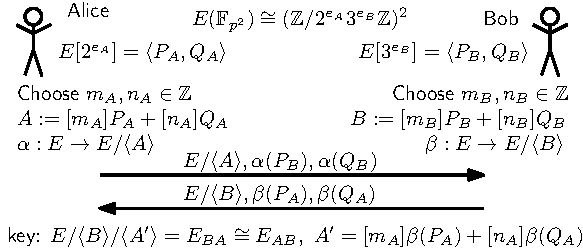
\includegraphics[width = \textwidth]{./sidh.pdf}
    \caption{\label{fig:sidh} The SIDH protocol for $l_A = 2$ and $l_B = 3$.}
\end{figure}

Note that these additional published points $\phi_A(P_B), \phi_A(Q_B), \phi_B(P_A), \phi_B(Q_A)$ make the security assumption required for SIDH somewhat nonstandard.
In particular, it is not enough to assume that the isogeny path problem is hard, and also if we relax this in an analogeous way to the classical Diffie-Hellman assumption (i.e. it is impossible to find $E_{AB}$ given $E_A$ and $E_B$) is not enough.
As it turns out, this additional information indeed decreases the security, as first mentioned by Cristophe Petit \cite{torsion_point_attack}.
However, it still was a big shock when \cite{sidh_broken} discovered an efficient attack using these torsion points, bringing the complete demise of SIDH.
This is even more surprising, as an SIDH-based cryptosystem named SIKE \cite{sike} was already considered a promising candidate for post-quantum crypto, and made it into the fourth (and final) round of the NIST post-quantum standardization process.

Since SIDH is broken, it does not serve perfectly to motivate the usefulness of a way to generate supersingular curves without revealing a trapdoor.
Still, we want to mention that choosing a starting curve with unknown endomorphism ring can prevent the torsion point attacks of \cite{torsion_point_attack}.
Next, we want to present another, slightly more exotic cryptosystem for which it is important to have a hard starting curve, i.e. a curve for which nobody knows a trapdoor (e.g. the endomorphism ring).

\section{An isogeny-based verifiable delay function}
\label{sec:verifiable_delay_function}
In this section, we present the verifiable delay function by De Feo, Masson, Petit and Sanso \cite{verifiable_delay_function}.
A \emph{verifiable delay function} (VDF) as first formalized in \cite{definition_verifiable_delay_function} is a cryptographic primitive consisting of three algorithms
\begin{itemize}
    \item \textbf{KeyGen}$(\lambda, T)$ takes a security parameter $\lambda$ and a time parameter $T$ and computes a pair $(\mathrm{ek}, \mathrm{vk})$ of an evaluation key $\mathrm{ek}$ and a verification key $\mathrm{vk}$.
    \item \textbf{Eval}$(\mathrm{ek}, s)$ takes the evaluation key and an input $s$ and computes an output $a$. 
    The key feature is that it should be impossible to compute \textbf{Eval} in time less than $T$, no matter how much parallel computing capabilities are available.
    \item \textbf{Verify}$(\mathrm{vk}, s, a)$ takes the verification key, the input $s$ and the output $a$ and checks whether \textbf{Eval}$(\mathrm{ek}, s) = a$.
\end{itemize}
Both \textbf{KeyGen} and \textbf{Verify} should run in time $O(\mathrm{poly}(\lambda))$, while \textbf{Eval} should (of course) run in time $T$.
The security of the VDF consists then of the three properties \emph{Correctness}, \emph{Soundness} and \emph{Sequentiality}.
As usual, correctness and soundness refer to the fact that \textbf{Verify} accepts correctly computed outputs (i.e. by \textbf{Eval}) and declines other outputs, both with probability $1 - 2^{-\lambda}$.
The interesting property is sequentiality, which states that it is impossible to compute \textbf{Eval}$(\mathrm{ek}, s)$ in less than $T$ computational steps, no matter how much parallel processing is available.

Therefore, a verifiable delay function provides a way of ensuring that an output $a$ is only known after a certain amount of wall clock time has elapsed (starting from the point at which the input $s$ is known).
Most applications focus on the use to generate public, trusted randomness: Some public entropy source provides the input $s$, but we assume that an attacker has ways to influence the entropy source (a common example are stock market prices).
To prevent an attacker from exploiting this, one now uses the entropy source $a = $ \textbf{Eval}$(\mathrm{ek}, s)$ instead, which can still be manipulated by the attacker, but not exploited anymore.
More concretely, if $T$ is larger than the natural change interval of the source $s$, an attacker cannot predict fast enough how a manipulation influences the output, and thus not profit from it.
There are more applications, for example in blockchain technology.

The isogeny-based VDF from \cite{verifiable_delay_function} relaxes this slightly by allowing the setup routine to take time $O(\mathrm{poly}(\lambda, T))$.
Apart from that, it satisfies above security properties under some isogeny-related security assumptions.
The basic idea is as follows.

The only efficient way we know to evaluate an isogeny $\psi: E \to E'$ of exponential degree $l^T$ is to write it as a sequence
\begin{equation*}
    E = E_0 \overset{\psi_1}{\longrightarrow} E_1 \overset{\psi_2}{\longrightarrow} \ ... \ \overset{\psi_T}{\longrightarrow} E_T = E'
\end{equation*}
of $l$-isogenies, and then compute the points $P_i = \psi_i(P_{i - 1})$ for an input point $P_0 \in E$.
Clearly, since $P_i$ depends on $P_{i - 1}$, it is impossible to effectively parallelize that.
Hence, it seems like a reasonable security assumption that $\psi(P)$ cannot be evaluated in less than $T$ time steps, and thus can be used for the function \textbf{Eval}.

Verification on the other hand can now be done using the Weil pairing.
If $P \in E[m]$ (with $m$ coprime to $l$ and $p$), we have that
\begin{equation*}
    e_m(\hat{\psi}(P), Q) = e_m(P, \psi(Q))
\end{equation*}
and (assuming that $\hat{\psi}(P)$ is known), we can compute $e_m(\hat{\psi}(P), Q)$ very efficiently.
There is just one problem here.
The map $e_m(P, \cdot): E[m] \to \mu_m$ obviously cannot be injective by a cardinality argument, and indeed, given $\psi(Q)$ we can easily compute other points $Q'$ with
\begin{equation*}
    e_m(P, \psi(Q)) = e_m(P, Q')
\end{equation*}
This obviously violates the soundness of system, as an attacker could compute $Q = $ \textbf{Eval}$(\mathrm{ek}, Q) = \psi(Q)$, but then claim $Q'$ to be the result.
Verification as above will not detect this.
To make it work, \cite{verifiable_delay_function} proposes to assume that $E/\F_p$ and use the trace map
\begin{equation*}
    \mathrm{Tr}: E[m] \to E[m] \cap E(\F_p), \quad P \mapsto P + \pi_E(P)
\end{equation*}
This map is $m$-to-1, and we have that
\begin{equation*}
    e_m(P, \mathrm{Tr}(\psi(Q))) = e_m(\hat{\psi}(P), Q)^2
\end{equation*}
which can be used for verification.
This now works, since the map $e_m(P, \cdot): E[m] \cap E(\F_p) \to \mu_m$ is indeed bijective for suitable choices of $P$.
Therefore, we get the scheme displayed in Algorithms~\ref{alg:setup_vdf}, \ref{alg:eval_vdf} and~\ref{alg:verify_vdf}.
\begin{algorithm}
    \caption{\label{alg:setup_vdf} \textbf{Setup}\\
    \textbf{Input:} A security parameter $\lambda$ and a time parameter $T$\\
    \textbf{Output:} Curves $E$ and $E'$, an evaluation key $\psi: E' \to E$ and a verification key $(P, \hat{\psi}(P))$}
    \begin{algorithmic}[1]
        \State Find distinct primes $p$ and $m$ of size depending on $\lambda$
        \State Find a random supersingular Elliptic Curve $E$ over $\F_p$
        \State Take a random walk of length $T$ starting from $E$ in the 2-isogeny graph, given by $\hat{\psi}: E \to E'$
        \State Find a random point $P \in E[m]$
        \State Compute $\hat{\psi}(P)$
        \State\Return $\mathrm{ek} = (E, E', \psi)$ and $\mathrm{vk} = (E, E', P, \hat{\psi}(P))$
    \end{algorithmic}
\end{algorithm}
\begin{algorithm}
    \caption{\label{alg:eval_vdf} \textbf{Eval}\\
    \textbf{Input:} The evaluation key $(E, E', \psi)$ and an input point $Q \in E'[m]$\\
    \textbf{Output:} An output point $Q' \in E[m]$}
    \begin{algorithmic}[1]
        \State Compute $\psi(Q)$
        \State\Return $Q' := \mathrm{Tr}(\psi(Q))$
    \end{algorithmic}
\end{algorithm}
\begin{algorithm}
    \caption{\label{alg:verify_vdf} \textbf{Verify}\\
    \textbf{Input:} The verification key $(E, E', P, \hat{\psi}(P))$, an input $Q \in E'[m]$ and an output $Q'$\\
    \textbf{Output:} An output point $\psi(Q)$}
    \begin{algorithmic}[1]
        \If{$Q' \in \mathrm{im}(\mathrm{Tr}) = E[m] \cap E(\F_p)$ and $e_m(P, Q') = e_m(\hat{\psi}(P), Q)^2$}
            \State\Return Valid
        \Else
            \State\Return Invalid
        \EndIf
    \end{algorithmic}
\end{algorithm}

In a practical implementation, we might want to exclude $P \in E[m]$ such that the map $e_m(P, \cdot): E[m] \cap E(\F_p) \to \mu_m$ is not bijective.
This is done in \cite{verifiable_delay_function}, but we will ignore those cases here.
Furthermore, we also will not prove that this is indeed a VDL, again refering the reader to \cite{verifiable_delay_function}.

However, we do want to discuss step 2 in the setup step, Algorithm~\ref{alg:setup_vdf}.
In particular, we claim that the curve $E$ has to be generated in a way that does not reveal its endomorphism ring $\End(E)$, or the resulting scheme will be insecure.
Hence, the classical methods of using CM techniques and random walks fail here.
Since there is currently no known alternative, at the moment this VDF requires a trusted party to generate the cuve $E$, and then forget about its endomorphism ring.

Namely, note that breaking sequentiality of the VDF can be achieved by solving the \emph{isogeny shortcut problem}.
\begin{problem}
    Given an isogeny $\psi: E \to E'$ of exponential degree $l^T$ and a point $Q \in E$, compute $\psi(Q)$ in time less than $T$.
\end{problem}
Since the supersingular isogeny graph is an expander, there exists always a path $E \to E'$ of length $O(\log(p))$.
Hence, if $T \in \omega(\log(p))$, we can solve the isogeny shortcut problem by the following three steps
\begin{itemize}
    \item Find an isogeny $\phi: E \to E'$ of degree at most $l^{O(\log(p))}$
    \item Find an endomorphism $\alpha \in \End(E')$ such that $\restr{\alpha \circ \phi}{E[m]} = \restr{\psi}{E[m]}$
    \item Evaluate $\alpha(\phi(P))$
\end{itemize}
Using similar techniques to the reductions between the isogeny path problem and the endomorphism ring problem \cite{endomorphism_ring_isogeny_path_equivalent}, the authors in \cite{verifiable_delay_function} have now shown that all three of these steps are indeed possible in time polynomial in $\log(T)$ if the endomorphism ring $\End(E)$ is known.
Hence, anyone who knows the endomorphism ring of the starting curve $E$ from Algorithm~\ref{alg:setup_vdf} can compute \textbf{Eval} in time less than $T$, thus breaking the protocol.

This is one of several examples why the generation of supersingular curves without revealing a trapdoor would be an important tool for cryptography.
However, as already mentioned, it is still an open problem to find an algorithm that achieves this.
In the next chapter, we will now present the progress we made on this problem. 

\chapter{Generating supersingular curves}


In this chapter, we now come to the main question of this work.
We have always talked about the ``generation of supersingular curves without revealing a trapdoor'', but in fact multiple variants of this problem are conceivable.
Following \cite{base_paper}, we thus define the following three problems.
For all of these problems, we are interested in an algorithm that runs in time polynomial in $\log(p)$.
\begin{problem}[Demonstrating a hard curve]
    Given a prime $p$, compute a supersingular curve $E$ over $\F_{p^2}$ without revealing $\End(E)$.
\end{problem}
We can formalize the requirement ``without revealing $\End(E)$'' as follows.
Given $E$ and any random bits passed to the generation algorithm, it should be impossible to compute $\End(E)$.
This of course excludes random walk-based methods, since the random bits used for the random walk allows us to repeat the walk, and so find an isogeny $E_0 \to E$ from the starting curve $E_0$.
Using that isogeny, we then can compute $\End(E)$ (assuming we know $\End(E_0)$).
Furthermore, it excludes methods that yield curves with very small endomorphism ring, as those endomorphism rings are always efficiently computable.

Note that an algorithm solving the hard curve demonstration problem does not have to be randomized.
In fact, it would already be interesting to find just a single hard curve over $\F_{p^2}$ for which nobody knows the endomorphism ring.
This is different for the next problem.
\begin{problem}[Generating a random hard curve]
    Given a prime $p$, compute a random supersingular curve $E$ uniformly selected from some exponentially sized set of supersingular curves over $\F_{p^2}$, without revealing $\End(E)$.
\end{problem}
In particular, a solution to the problem can then be used to setup any cryptographic primitive with hard and secure starting curves.

Finally, the most difficult problem is to find a trapdoor-free hash function to the whole set of supersingular curves.
\begin{problem}[Hashing into hard curves]
    Given a prime $p$ and an input string $s$, deterministically find a supersingular curve $E$ without revealing $\End(E)$.
    Furthermore, if $s$ is uniform on $\{0, 1\}^n$ for a sufficiently large $n$, the resulting curve $E$ should be uniform among all supersingular curves over $\F_{p^2}$.
\end{problem}
An algorithm solving the above problem can then easily be made into a collision-free hash function by prepending it with a secure hash function.
Note that for most applications, it would already be sufficient if the above problems could be solved only for certain primes $p$. 

Next, we want to present some of the known methods to generate supersingular elliptic curves, and discuss why (or why not) they can solve one of the above problems.
After that, we introduce the idea of Katherine Stange, which is the second proposal of \cite{base_paper}.
We discuss both the theoretical and implementation issues in detail, and then prove our main result, Prop.~\ref{prop:main_result1}.
Finally, we present a modified version and prove some results on the associated distribution of supersingular curves, which includes our second main result, Prop.~\ref{prop:main_result2} and an analysis of another case.
We conclude by giving an idea that might help with performing the computations that go with our modified approach efficiently. 

\section{Naive and classical approaches}
\label{prop:naive_classical_approaches}
First, we have a look at some simple or well-known approaches to the problem, to get a feeling for the challenges.

\paragraph{Random Sampling} It is a folklore knowledge that all supersingular curves over $\bar{\F}_p$ have a j-invariant in $\F_{p^2}$, i.e. are isomorphic to a curve defined over $\F_{p^2}$.
Hence, the most naive approach is to sample random $j \in \F_{p^2}$ and check if they define supersingular curves.
It is clear that this algorithm does not reveal any information about isogenies or the endomorphism ring of the found curve, unless the information can be efficiently computed from the curve itself (in which case the cryptographic schemes are broken anyway).
However, the number of supersingular curves over $\F_{p^2}$ is only approximately $p/12$, which means that the expected number of required samples (and supersingularity checks) is about $12p$, which is exponential in $\log(p)$.

\paragraph{Random Walk} Opposed to that we have the way supersingular curves are currently generated:
As discussed in Section~\ref{sec:supersingular_isogeny_graph}, a random walk of length polynomial in $\log(p)$ in the supersingular $l$-isogeny graph is sufficient to find an (almost) uniformly distributed supersingular curve.
As long as we know one fixed curve to start with, this is quite efficient.
However, clearly this computation reveals a power-$l$ degree isogeny to the fixed starting curve, which is exactly what we want to avoid.

\paragraph{CM methods} Using the theory of complex multiplication of curves over $\C$ and their reduction modulo primes, Brökner \cite{constructing_supersingular_curves} found an algorithm that can find supersingular curves $E$ over $\F_p$, even for astronomically large primes $p$.
This method is often combined with random walks, as these naturally require a supersingular curve to start the walk from.

However, curves generated with Brökner's method have one drawback.
Namely, the algorithm has time complexity polynomial in the discriminant of the endomorphism ring of the considered curves over $\C$, and this endomorphism ring embeds into the endomorphism ring of their reduction mod $p$.
Hence, it is only efficient when generating curves with very small endomorphism rings.
This is clearly a weakness, as small endomorphism rings can be computed efficiently, for example by an exhaustive search of all low-degree isogenies.

\paragraph{Polynomial with supersingular roots} An idea that is more similar to what we will do next, is to use the following theorem \cite[Thm~V.4.1]{arithmetic_elliptic_curves}.
\begin{prop}
    Let $p$ be an odd prime and $m = (p - 1)/2$. Then the elliptic curve given by $y^2 = x(x - 1)(x - \lambda)$ over $\F_q$ is supersingular, if and only if
    \begin{equation*}
        H_p(\lambda) := \sum_{i = 0}^m {m \choose i}^2 \lambda^i = 0
    \end{equation*}
\end{prop}
In other words, we just have to find a random root of the polynomial $H_p(X)$, which then gives rise to a random supersingular curve.
The obvious problem here is again that $p$ is exponential in the input size $\log(p)$, thus the polynomial $H_p(X)$ also has exponential degree, and it is not clear if we can find a random root efficiently.

In fact, the first idea in \cite{base_paper} tries to find a random root of this polynomial, by a method similar to the Newton-Raphson iteration.
Of course, this is challenging, because it is not even clear how to evaluate $H_p(\lambda)$ efficiently for a given $\lambda$.

\section{Katherine Stange's approach}
In our research, we mainly focused on analyzing and improving the second proposal in \cite{base_paper}, which was proposed by Katherine Stange.
It is based on the following intuition.

Since the supersingular isogeny graph is an expander, it is relatively likely that there is an $n$-isogeny between two random curves $E$ and $E'$ (for a fixed $n$).
On the other hand, this is much less likely in the ordinary case.
We expect that this still applies when we take not two random curves, but a random curve $E$ and its Frobenius conjugate $E^{(p)}$, i.e. the curve with j-invariant $j(E)^p$.
Hence, the roots of
\begin{equation*}
    \Phi_n(X, X^p)
\end{equation*}
should contain a relatively large fraction of supersingular roots over $\F_{p^2}$.
This fraction can be increased by taking e.g. a gcd like
\begin{equation*}
    f_{p, n, m} := \gcd(\Phi_n(X, X^p), \Phi_m(X, X^p))
\end{equation*}
Hence, computing a random root of such a polynomial might give us a hard supersingular curve.
This idea leads to two main open questions:
\begin{question}
    \label{question:first}
    How large is the fraction of supersingular roots of $\Phi_m(X, X^p)$ resp. $f_{p, n, m}$ among all roots in $\F_{p^2}$?
\end{question}
In particular, for the method to have any hope of success, we require the fraction to be at least $1/\mathrm{poly}(\log(p))$.

The second question is more implementation-oriented. 
\begin{question}
    \label{question:second}
    How can we efficiently compute $f_{p, n, m}$, especially if $n$ resp. $m$ are exponentially large?
    Or can we efficiently find a root in some other way?
\end{question}
In the following, we try to answer both questions.
First, we present the special case that $n = l^e$ is a prime power, and describe how this might help with computing a root of $f_{p, n, m}$.
We then explain how we might be able to use the class group action to find the fraction of supersingular roots.
Finally, we present our first main result, which answers Question~\ref{question:first} for a subset of the $m$ and $n = l^e$.
Our approaches for an efficient computation also apply to this special case.
However, we are not able to answer Question~\ref{question:second}, and only provide some hints and ideas how one might handle certain difficulties.

In the case that both $n$ and $m$ are small (i.e. polynomial in $\log(p)$), \cite{base_paper} presents an approach that can find roots of $f_{p, n, m}$ even though $p$ is exponentially large, so $\Phi_n(X, X^p)$ and $\Phi_n(X, X^p)$ have exponential degree.
The idea is to take a non-square in $\F_p$ and its square root $\delta \in \F_{p^2}$.
Then $(a + b\delta)^p = a - b\delta$ and so we can equivalently look for $x, y \in \F_p$ such that
\begin{equation*}
    \Phi_n(x + \delta y, x - \delta y) = \Phi_m(x + \delta y, x - \delta y) = 0
\end{equation*}
Hence, we look for a root in $\F_p$ of the polynomial
\begin{equation*}
    \mathrm{res}_Y(\Phi_n(X + \delta Y, X - \delta Y), \Phi_m(X + \delta Y, X - \delta Y))
\end{equation*}
Of course, for each such root $x$ we still have to check that
\begin{equation*}
    \Phi_n(x + \delta Y, x - \delta Y) \quad \text{and} \quad \Phi_m(x + \delta Y, x - \delta Y)
\end{equation*}
also have roots in $\F_p$.
All of this is possible, since the polynomials in each case have degree polynomial in $n$ resp. $m$.

However, note that the elliptic curve corresponding to a root of $f_{p, n, m}$ will have an endomorphism of degree $nm$.
If we choose both $n$ and $m$ of size polynomially large in $\log(p)$, this means the endomorphism ring has polynomial discriminant, which is a weakness.
Hence, at least one of $n$ resp. $m$ has to be super-polynomial (or better exponential) in $\log(p)$.

This of course makes it very hard to even write down or compute some properties of $\Phi_n$.
In particular, the above approach does not work anymore.
We will now study a slight modification and focus on the case that $n = l^e$ is a prime power, in which we can circumvent at least parts of the problem.

\subsection{The prime power case}
First of all, we describe how the assumption $n = l^e$ might help us to work with $\Phi_n$.
Note that $\Phi_{l^e}(j(E), j(E'))$ is equivalent to there being a cyclic $l^e$-isogeny between $E$ and $E'$.
If we relax this to just any $l^e$-isogeny and note that an $l^e$-isogeny is equal to an $l$-isogeny path of length $e$, we can instead work with the condition
\begin{equation*}
    \exists x_1, ..., x_{e - 1}: \ \Phi_l(x, x_1) = \Phi_l(x_1, x_2) = ... = \Phi_l(x_{e - 1}, y) = 0
\end{equation*}
In other words, we look for a solution to the polynomial system
\begin{equation*}
    F_{p, m, l^e} := \langle \Phi_m(x, x^p), \Phi_l(x, x_1), ..., \Phi_l(x_{e - 1}, x^p) \rangle
\end{equation*}
Of course, we can again take a non-square of $\F_p$ and its root $\delta \in \F_{p^2}$ and write $x_i = y_i + \delta z_i$.
Hence, we look for a solution in $\F_p$ of the system
\begin{equation*}
    \langle \Phi_m(y + \delta z, y - \delta z), \Phi_l(y + \delta z, y_1 + \delta z_1), ..., \Phi_l(y_{e - 1} + \delta z_{e - 1}, y - \delta z) \rangle
\end{equation*}
This polynomial system is now at least efficiently computable and representable (using a standard, i.e. non-sparse, representation).

The other advantage of this approach is that every supersingular curve $E$ has an $l^e$-isogeny to $E^{(p)}$ if $e \in \Omega(\log_l(p))$.
This follows from the presented results on expander graphs.
More concretely, Theorem~\ref{prop:supersingular_graph_ramajuan} shows that the supersingular $l$-isogeny graph over $\F_{p^2}$ is an $\epsilon$-expander for
\begin{equation*}
    \epsilon = 1 - \frac {2\sqrt{d - 1}} d = 1 - 2 \frac {\sqrt{l}} {l + 1} \geq 1 - \frac 2 {\sqrt{l}}
\end{equation*}
Thus, a random walk of length at least
\begin{equation*}
    -\log_{2/\sqrt{l}}(p/12) \leq 2 \log_l(p) = \Theta(\log_l(p))
\end{equation*}
has a nonzero probability of ending in any fixed vertex, by Prop.~\ref{prop:expander_random_walk}.

This leaves us with a polynomial system of $O(\log(p))$ unknowns and equations, which at least can be explicitly written down.
Now we want to study how big the fraction of supersingular roots is.
We use the following corollary from the OSIDH class group action, see e.g. \cite[Thm~4.3]{chenu_smith}.
\begin{corollary}
    \label{prop:osidh_class_group_action}
    There are $\Theta(\sqrt{mp})$ supersingular curves $E$ over $\F_{p^2}$ with an $m$-isogeny to $E^{(p)}$.
\end{corollary}
To begin with, by our choice of $e = \Theta(\log_l(p))$, we can assume that all supersingular j-invariants are roots of $\Phi_{l^e}(X, X^p)$, and so the number of supersingular roots is $O(\sqrt{mp})$, by the above Corollary~\ref{prop:osidh_class_group_action}.
Hence, we want to find instances of $l, e$ and $m$ such that above system has only a small amount of ordinary roots, preferably $o(\sqrt{mp})$. 

\subsection{Studying the number of ordinary roots}
To estimate the number of ordinary roots, we will of course use the class group action.
Thus, we need a bound on the class number of quadratic imaginary orders.
The next theorem puts together some classical results, in particular the famous class number formula (see e.g. \cite[Corollary~VII.5.11]{neukirch}).
\begin{theorem}
    \label{prop:class_number_bounds}
    Let $\O$ be an order in a quadratic imaginary number field with discriminant $D = d(\O)$.
    Assuming GRH, we then have for the class number $h(D) := \#\Cl(\O)$ that
    \begin{equation*}
        \Theta\left(\frac {\sqrt{|D|}} {(\log\log|D|)^2}\right) \leq h(D) \leq \Theta\left(\sqrt{|D|} (\log|D|)^2\right)
    \end{equation*}
\end{theorem}
\begin{proof}
    We assume wlog that $d_K := d(\O_K) < -4$.
    Then the Dirichlet class number formula has the form
    \begin{equation*}
        h(\O_K) = \frac {\sqrt{|d_K|}} {2\pi} L(1, \chi)
    \end{equation*}
    where
    \begin{equation*}
        \chi: \Z \to \C, \quad m \mapsto \left(\frac d m\right)
    \end{equation*}
    is a real Dirichlet character and $L(s, \chi)$ is its Dirichlet L-function.
    This follows from the general class number formula, as e.g. presented in \cite[Korollar~VII.5.11]{neukirch}.

    In \cite[Thm~1]{class_number_lower_bound}, it was proven under GRH that $L(1, \chi) \geq \Theta(\sqrt{|d_K|}\log\log|d_K|)$, and the lower bound for $\O_K$ follows.
    The upper bound can easily be proven via partial summation, and does not require GRH.
    Hence, for a maximal order, we have
    \begin{equation*}
        \Theta\left(\frac {\sqrt{|D|}} {\log\log|D|}\right) \leq h(D) \leq \Theta\left(\sqrt{|D|} \log|D|\right)
    \end{equation*}

    To transfer this result to all orders, we use Corollary~\ref{prop:class_group_order}, from which it follows that
    \begin{equation*}
        h(\O) = h(\O_K) \frac {\#(\O_K / \mathfrak{f})^*} {\#(\O / \mathfrak{f})^*}
    \end{equation*}
    where $\mathfrak{f} = f\O_K \leq \O_K$ is the largest ideal contained in $\O$.
    By Corollary~\ref{prop:unit_fraction_bound}, we now see that
    \begin{equation*}
        \phi(f)h(\O_K) \leq h(\O) \leq \psi(f)h(\O_K)
    \end{equation*}
    It is a well-known fact that $\phi(f)$ is lower bounded by $\Omega(f/\log\log(f))$, and in \cite{upper_bound_dedekind_psi} it was shown that also $\psi(f)$ is upper bounded by $O(f\log\log(f)) \leq O(f\log(f))$.
    The claim now follows, since $\sqrt{|D|} = f \sqrt{|d_K|}$.
\end{proof}
Now let us come back to our estimate of the number of ordinary roots of $f_{p, m, n}$ resp. our polynomial system $F_{p, m, l^e}$.
First, we now explain why instead of (isomorphism classes of) curves it suffices to count endomorphism rings.

Whenever we have two ordinary curves $E$ and $E'$ with same endomorphism ring $\O$ in a quadratic imaginary number field $K$, then by the class group action, there is $\a \leq \O$ with $[\a].E = E'$.
Denote by
\begin{equation*}
    \Ell(\O) := \{ \text{$E$ elliptic curve} \ | \ \End(E) \cong \O \}
\end{equation*}
the set of elliptic curves with endomorphism ring $\O$.
Now the subgraph $G$ of $\Gamma_l(\F_q)$ induced by all the connected components of curves in $\Ell(\O)$ is a collection of isomorphic volcanoes.
The reason for this is the volcano structure theorem, Theorem~\ref{prop:isogeny_vulcano}, from which it follows that the structure of a volcano is determined just by the endomorphism ring of the curves on its crater.

Now consider the map
\begin{equation*}
    \Ell(\O) \to \Ell(\O), \quad E \mapsto [\a].E
\end{equation*}
It is not hard to see that this extends to a graph automorphism of $G$, again by the volcano structure.
However, it will then be not just a graph automorphism (i.e. preserves the graph structure), but also preserves Frobenius conjugates and the property of being defined over $\F_p$.
The latter follows, since being defined over $\F_p$ is a property of the endomorphism ring, namely equivalent to the ideal $(p, \pi)$ being principal.

Since our approach only uses properties of the $l$-isogeny graph and Frobenius conjugates, this means that if $E$ and $E'$ have the same endomorphism ring, it holds
\begin{equation*}
    f_{p, n, m}(j(E)) = 0 \quad \Leftrightarrow \quad f_{p, n, m}(j(E')) = 0
\end{equation*}
and similar for the system $F_{p, n, l^e}$.

Hence, we determine the set of endomorphism rings such that any (or equivalently all) corresponding curves are roots of the polynomials.
Then, the total number of curves is given by the sum over the class numbers $\sum_D h(D)$ where $D$ runs through the discriminants of said endomorphism rings. 

We mentioned before that $\Phi_m(X, X^p)$ has about $mp$ ordinary roots over $\bar{\F}_p$, but the argument implicitly assumed that the polynomial is separable.
Using endomorphism rings, it is now easy to properly lower bound the number of ordinary roots of $\Phi_m(X, X^p)$, as these correspond to the endomorphism rings with cyclic
\footnote{An element $\alpha \in \O$ is cyclic if the corresponding endomorphisms of curves $E$ with $\End(E) \cong \O$ are cyclic. This is equivalent to $n \notdivides \alpha$ for all $n \geq 2$.}
elements of norm $mp$. 
The reason is that this is equivalent to there being a solution $x \perp y$ of the Diophantine equation
\begin{equation*}
    x^2 + g y^2 = m p
\end{equation*}
where $\End(E) \cong \Z[\sqrt{g}]$, i.e. $D := d(\End(E)) = 4g$.
Note that we want a lower bound (we have an upper bound by the degree argument), and so we can ignore the possibilities in which $\End(E)$ is not of this form (i.e. $\End(E) \cong \Z[(1 + \sqrt{g})/2]$).

Furthermore, at the moment we content ourselves with a very crude estimate, but note that everything can be made rigorous.
We do that later with a very similar argument in Prop.~\ref{prop:counting_fp2_vulcano_levels}.
Neglecting $\log$-factors, we now have
\begin{align*}
    &\#\{ j \in \bar{\F}_p \ | \ \Phi_m(j, j^p) = 0 \} \geq \sum_{\substack{\text{$x^2 - gy^2 = mp$ solvable}\\\text{with $x \perp y$}}} h(4g) \\
    \geq& \sum_{0 < x < \sqrt{mp}} h(4x^2 - 4m p) \approx \sum_{0 < x < \sqrt{mp}} 2\sqrt{mp - x^2} \\
    \approx& \ 2\int_0^{\sqrt{mp}} \sqrt{mp - x^2} dx = 2mp \int_0^1 \sqrt{1 - x^2} dx \in \Omega(m p)
\end{align*}
None of the ways we consider to capture supersingularity by modular polynomials can completely exclude ordinary roots.
This is because an ordinary curve defined over $\F_p$ with endomorphisms of degree $m$ and $l$ will always be a root.
Similar situations can occur with other polynomial systems, but it is always the case that these ordinary curves have very small endomorphisms.
The next statement shows that this is not a problem, as those ordinary roots are very rare.
\begin{prop}
    \label{prop:small_endomorphism_rare}
    For $n > 0$, there are at most $O(n^{3/2}\log(n)^2)$ isomorphism classes of ordinary curves who have a non-integer endomorphism of degree $n$.
\end{prop}
\begin{proof}
    Assume that $\O$ is an imaginary quadratic order with $p \notdivides d(\O)$ that has a non-integer element $\beta \in \O \setminus \Z$ of norm $n$.
    The discriminant of the order $\Z[\beta]$ is $d(\Z[\beta]) = \mathrm{Tr}(\beta)^2 - 4\Norm(\beta) \geq -4\Norm(\beta)$.
    Hence $|d(\O)| \leq 4n$, and we find that the number of isomorphism classes of ordinary curves with a non-integer $n$-endomorphism is bounded by
    \begin{align*}
        \sum_{\substack{-4n \leq D \leq 0\\\mathclap{\text{$D$ fundamental discriminant}}}} h(D) \leq \sum_{1 \leq D \leq 4n} \sqrt{D}\log(D)^2 \in O(n^{3/2}\log(n)^2)
    \end{align*}
    This shows the claim.
\end{proof}
This is now as far as we can go in the general case.
The main problem is that once we want to determine which endomorphism rings have non-integer endomorphisms of two different degrees (e.g. $m$ and $l^e$), there is no analogue of the simple statement
\begin{equation*}
    \{ d(\O) \ | \ \text{$\O$ has cyclic endomorphism of degree $m$}\} \supseteq \{ 4(m - x^2) \ | \ 0 < x < \sqrt{m} \}
\end{equation*}
and an appropriate converse.

While the Diophantine equation $x^2 + \frac D 4 y^2 = m$ has been thoroughly studied (see e.g. \cite{cox_primes_of_form}), the best characterization for it being solvable (assuming $m = p$ is prime) involves the so-called Hilbert class polynomial
\begin{equation*}
    h_D(x) = \prod_{d(\End(E)) = D} (X - j(E))
\end{equation*}
In our case, $D$ is variable, which makes working with Hilbert class polynomials very unwieldy.
All in all, it seems like the general case is very hard to get a handle on.

\subsection{A working example}
While we are unlikely to get nice provable bounds on the number of ordinary roots in the general situation of $F_{p, m, l^e}$, there are special cases in which this is possible.
In particular, if we choose $m$ such that there is a simple relationship between $\Phi_m$ and $\Phi_{l^e}$, we can do something.
One situation in which everything works out is presented next.
In contrast to most of the other arguments we make in this section, here we argue (almost) solely with the structure of isogeny volcanoes.
\begin{prop}
    Let $l$ be a prime and further $f$ be odd and $e$ be even.
    Then the system
    \begin{equation*}
        F_{p, l^f, l^e} := \langle \Phi_{l^f}(x, x^p), \Phi_l(x, x_1), ..., \Phi_l(x_{e - 1}, x^p) \rangle
    \end{equation*}
    has $O(l^{3f}\log(l^f)^2)$ ordinary roots in $\F_{p^2}$
    \footnote{It might be not totally clear what we mean by an ordinary root of the system.
    So let us define the number of ordinary roots as the number of $j \in \bar{\F}_p$ such that $F_{p, l^f, l^e}(j, x_1, ..., x_{e - 1})$ has a solution.
    However, note that for a fixed $j$, the number of different solutions of the system is polynomial, hence it would not make a big difference if we counted all solution tuples $(x, x_1, ..., x_{e - 1})$.}.
\end{prop}
\begin{proof}
    We show that every ordinary root $j \in \F_{p^2}$ of $F_{p, l^f, l^e}$ has an endomorphism of degree at most $l^{2f}$ and the claim follows by Prop.~\ref{prop:small_endomorphism_rare}.

    For any ordinary curve $E$, denote now by $E_R$ the unique vertex in the crater of the $l$-isogeny volcano of $E$ that is connected to the lava flow tree of $E$ (in particular, $E_R = E$ if $E$ already lies on the crater).
    In other words, if $E$ is on the $i$-th lava flow tree level, then there is a sequence of ascending $l$-isogenies
    \begin{equation*}
        E = E_0 \to E_1 \to ... \to E_i = E_R
    \end{equation*}
    and $\End(E_R)$ is maximal at $l$ (meaning $l \notdivides [\O_{\End(E_R) \otimes \Q} : \End(E_R)]$).

    Note further that $(E^{(p)})_R = E_R^{(p)}$ for all ordinary curves $E$, by the functoriality of $\cdot^{(p)}$.

    Now assume a root $j$ of $F_{p, l^f, l^e}$ gives an ordinary curve $E$.
    We distinguish two cases.

    \begin{figure}
        \begin{center}
            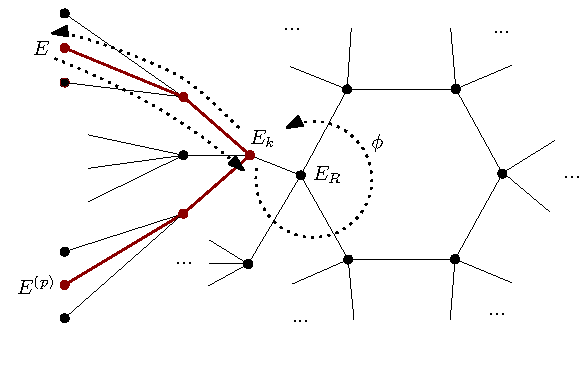
\includegraphics{./vulcano_sketch2.pdf}
        \end{center}
        \caption{\label{fig:fp_case}
            A sketch of the volcano in the case that $j(E_R) \in \F_p$ but $j(E) \notin \F_p$.
            The dotted path up to $E_k$ is then a small endomorphism of $E$, since we assume that $\phi$ is small.
            Furthermore, the path does not backtrack, as $\phi$ is cyclic and nontrivial.
        }
    \end{figure}

    If $j(E_R) \in \F_p$, i.e. the crater of the volcano is defined over $\F_p$, then clearly $E_R = (E^{(p)})_R$ (displayed in Figure~\ref{fig:fp_case}).
    Now let $k$ be minimal such that $j(E_k) \in \F_p$.
    Then every cyclic isogeny $E \to E^{(p)}$ has the form
    \begin{equation*}
        E \to E_1 \to ... \to E_k \ \overset{\phi}{\longrightarrow} \ E_k = E_k^{(p)} \to E_{k - 1}^{(p)} \to ... \to E^{(p)}
    \end{equation*}
    where $\phi$ is a power-of-$l$ endomorphism of $E_k$.

    If we apply this to the $l$-isogeny path $E \to E^{(p)}$ of length $f$, we see that $\phi$ is an $l^{f - 2i}$-endomorphism of $E_i$.
    However, since $f - 2i$ is odd by assumption, $\deg(\phi)$ is not a square and so $\phi$ is not an integer.
    This now gives a non-integer endomorphism
    \begin{equation*}
        E \to E_1 \to ... \to E_i \ \overset{\phi}{\longrightarrow} \ E_i \to E_{i - 1} \to ... \to E
    \end{equation*}
    of $E$ with degree $l^f$ and we are done.

    If $j(E_R) \notin \F_p$, then $E_R \not\cong E^{(p)}_R$.
    In particular, this means that the ideal $(p, \pi)$ in $\O := \End(E_R)$ is non-principal.
    Now we consider the subcases how $(l)$ splits in $\O$.
    
    \begin{figure}
        \begin{center}
            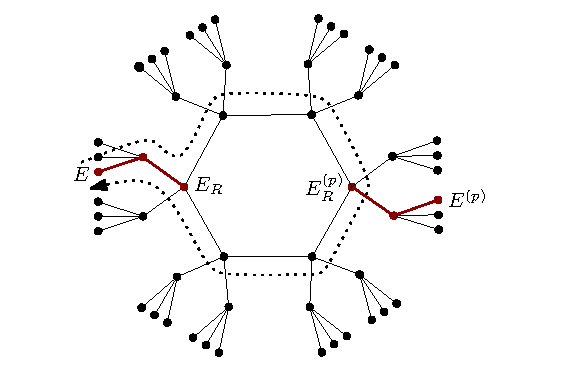
\includegraphics{./vulcano_sketch1.pdf}
        \end{center}
        \caption{\label{fig:split_case} 
            A sketch of the volcano in the case that $j(E_R) \in \F_{p^2} \setminus \F_p$ and $l$ splits in $\O_K$.
            Since $E_R$ is defined over $\F_{p^2}$, we know that $[(p, \pi)]^2.E_R = E_R$ and so $E_R^{(p)}$ is on the opposite side of the volcano.
            Now we can take the dotted path around the crater and find a small endomorphism of $E$.
        }
    \end{figure}

    If $(l) = \l_1 \l_2$ is split in $\O$ (see also Figure~\ref{fig:split_case}), note that our cyclic $l$-isogeny path $E \to E^{(p)}$ of length $f$ induces a path $E_R \to E_R^{(p)}$ of length $f - 2i$, for some $i \geq 0$.
    Since walking around the crater is given by the action of $\l_1$, we see that $[(p, \pi)] = [\l_1]^{f - 2i}$ in the ideal class group.
    Thus $\l_1^{2f - 4i}$ is principal ($E_R$ is defined over $\F_{p^2}$, so $[(p, \pi)]^2 = 1$), and its generator gives a non-integer endomorphism $\phi$ of $\End(E_R)$ of degree $l^{2f - 4i}$.
    Now
    \begin{equation*}
        E = E_0 \to E_1 \to ... \to E_i = E_R \ \overset{\phi}{\longrightarrow} E_R = E_i \to E_{i - 1} \to ... \to E
    \end{equation*}
    gives a non-integer endomorphism of $E$ with degree $l^{2f - 2i} \leq l^{2f}$, so we are done.

    If $(l)$ is inert in $\O$, the crater only has a single vertex.
    Since we have $E_R \not\cong E_R^{(p)}$ are both curves in a crater, we see that they must be in different $l$-isogeny volcanoes.
    Hence, this also holds for $E$ and $E^{(p)}$ and there cannot be an $l^f$-isogeny $E \to E^{(p)}$, contradicting our assumption.

    Finally, we are left with the case that $(l) = \l^2$ is ramified in $\O$ (see Figure~\ref{fig:ramified_case}).
    This is the only case where we will use the fact there is also an $l$-isogeny path $E \to E^{(p)}$ of length $e$.
    Since $(l)$ is ramified, we see that the crater of the volcano has exactly two vertices, which then must be $E_R$ and $E_R^{(p)}$.

    \begin{figure}
        \begin{center}
            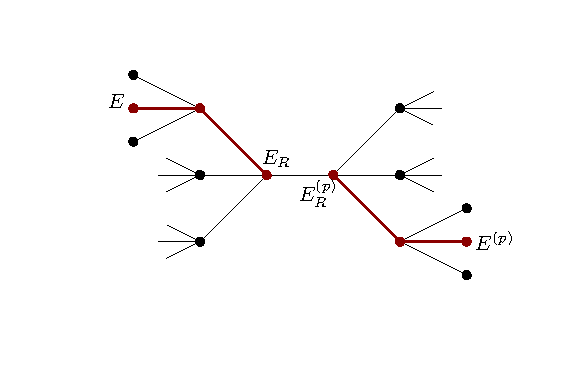
\includegraphics{./vulcano_sketch3.pdf}
        \end{center}
        \caption{\label{fig:ramified_case}
            A sketch of the volcano in the case that $j(E_R) \in \F_{p^2} \setminus \F_p$ and $l$ is ramified in $\O_K$.
            In this graph, there is no path from $E$ to $E^{(p)}$ of even length.
        }
    \end{figure}

    We did not assume that the $l$-isogeny path $E \to E^{(p)}$ of length $e$ does not backtrack.
    But we can still remove the backtracks, and get a cyclic path $E \to E^{(p)}$ of length $e - 2k$, where $k$ is the number of backtracking steps in the original path.
    Now this new path must go through the crater, and thus is of the form
    \begin{equation*}
        E = E_0 \to E_1 \to ... \to E_i = E_R \to E_R^{(p)} = E_i^{(p)} \to E_{i - 1}^{(p)} \to ... \to E_0^{(p)} = E^{(p)}
    \end{equation*}
    However, now we get a contradiction, since above path has odd length $2i + 1$, while $e - 2k$ is even by assumption.
\end{proof}
By choosing $e = \Theta(\log_l(p))$, we have $\Theta(\sqrt{l^fp})$ supersingular roots of above system.
Thus, this theorem shows that the fraction of supersingular roots is not just noticeable, i.e. $1/\mathrm{poly}(\log(p))$, but even exponentially large.
In particular, this proves our main result Prop.~\ref{prop:main_result1} and answers Question~\ref{question:first} in the considered case.
Furthermore an algorithm that is able to efficiently compute a random root of $F_{p, l^f, l^e}$ over $\F_{p^2}$ can be used to generate a random supersingular curve with very high probability.
We expect that this will not reveal a trapdoor, i.e. information about the endomorphism ring.

Note that we can choose $f$ very small, e.g. $\log_l\log(p)$ and thus $n = l^f$ is polynomial in $\log(p)$.
Therefore, we can indeed write down the system
\begin{equation*}
    F_{p, l^f, l^e} := \langle \Phi_{l^f}(x, x^p), \Phi_l(x, x_1), ..., \Phi_l(x_{e - 1}, x^p) \rangle
\end{equation*}
explicitly.
Next, we try to demonstrate this in one example.
\begin{example}
    Assume we choose $p = 51$, $l = 3$, $f = 3$ and $e = 4$.
    Then $e$ is somewhat smaller than the bound required to have $\Phi_{l^e}(j_1, j_2) = 0$ for all supersingular $j_1$, $j_2$.
    Still, we expect that most roots of $f_{p, l^f, l^e}$ are supersingular.
    We have that
    \begin{align*}
        \Phi_3 =& -x^3y^3 + 6x^3y^2 + 6x^2y^3 + x^4 + 8x^3y + 7x^2y^2 + 8xy^3 + y^4 + 9x^3 \\
        &+ 12x^2y + 12xy^2 + 9y^3 - 26x^2 + 5xy - 26y^2 - 26x - 26y
    \end{align*}
    and hence, $\Phi_{l^f}$ and $\Phi_{l^e}$ are huge, having 1240 resp. 11162 monomials.
    However, we can still compute $f_{p, l^f, l^e}$, which is a polynomial of degree $156$.
    It has the $F_{p^2}$-roots
    \begin{equation*}
        39, 52\alpha + 42, \alpha + 38, 0, 46, 44\alpha + 46, 9\alpha + 10, 50
    \end{equation*}
    Of those, $0$, $50$, $46$, $9\alpha + 10$ and $44\alpha + 46$ are supersingular, and the other three are ordinary.
    The corresponding $3$-isogeny graphs are displayed in Figure~\ref{fig:example_51}.
    Note that all ordinary solutions are in a volcano with a curve that has a non-integer $3$-endomorphism.
    \begin{figure}
        \begin{minipage}{0.5\textwidth}
            \centering
            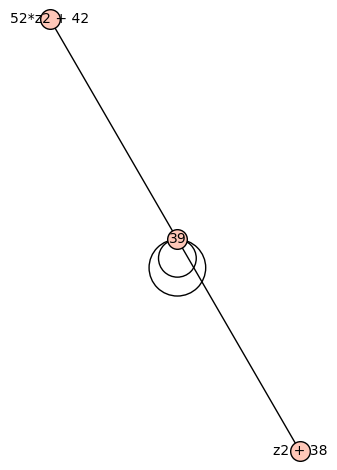
\includegraphics[width = 0.75\textwidth]{../example_51_ordinary.png}
        \end{minipage}%
        \begin{minipage}{0.5\textwidth}
            \centering
            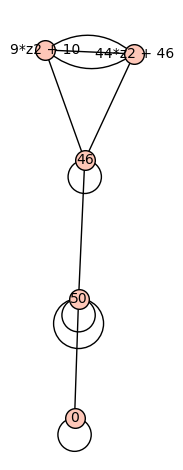
\includegraphics[width = 0.45\textwidth]{../example_51_supersingular.png}
        \end{minipage}
        \caption{\label{fig:example_51} Ordinary 3-isogeny volcano (left) and supersingular 3-isogeny graph (right) over $\F_{51^2}$, where $\mathrm{z2} = \alpha$ is a generator of $\F_{51^2}$.}
    \end{figure}
\end{example}
It is a fact that this example cannot completely show that the method works, and most roots are supersingular.
It would be much preferable if we could choose larger parameters, such that $\sqrt{p}$ and polynomial in $\log(p)$ look very different.
However, we very soon hit the limits of computers - just remember that $\Phi_{3^4}$ already has 11162 monomials.

Also the standard approach using Groebner basis does not work, as we expect its complexity to be exponential in the number of variables, i.e. exponential in $\log_l(p)$.
Already for $l = 3$ and $e = 4$, it is very slow and takes time in the range of minutes.
The original paper~\cite{base_paper} mentioned it might be possible to use a ``square-and-multiply'' approach to compute the resultant
\begin{equation*}
    \mathrm{res}_Y(\Phi_n(X + \delta Y, X - \delta Y), \Phi_{l^e}(X + \delta Y, X - \delta Y))
\end{equation*}
for some $\delta = \sqrt{a}$ with a non-square $a \in \F_p^*$.
However this means we will not represent $\Phi_{l^e}$ by the polynomial system anymore, hence we would need to get enough information about the exponential-degree modular polynomial $\Phi_{l^e}$ another way.
This seems to be a very serious obstacle.

\section{An idea based on Sutherland's supersingularity test}
As an alternative to the above approach, we propose another set of polynomial equations, whose properties might make computations easier.
In particular, our system does not consist of long dependency cycles, in the sense that we have equations $f_i(x_i, x_{i + 1})$ and $f_n(x_n, x_0)$.
Instead, our equations are of the form $f_i(x_i, x_{i + 1})$ and $f_n(x_n)$, which seems to be easier to handle.

The basic idea is to use Sutherland's supersingularity test (see Section~\ref{sec:sutherlands_supersingularity_test}).
Namely, if we take three non-backtracking walks away from an ordinary starting curve $E_0$ (such that the second vertices are distinct), then at least one of them will descend into a lava flow, and encounter a curve not defined over $\F_{p^2}$ after polynomially many steps.
On the other hand, if we do the same starting from a supersingular curve, this will not happen, as the whole supersingular isogeny graph is defined over $\F_{p^2}$.

We have already seen that $\log_l(p)$ steps are sufficient, which is also Sutherland's original choice.
However, this is not optimal, and in our case, we are also interested in how many ordinary curves we will accept if we choose $n$ smaller than the optimal bound.
In particular, our method can deal with a small number of ordinary roots (e.g. polynomially many), it should just not exponentially exceed the number of supersingular roots.
All this is considered in the next two propositions, which are again phrased in the language of endomorphism rings.
\begin{prop}
    \label{prop:frobenius_in_nonmaximal_order}
    Let $p$ be an odd prime and $m \geq 2$ an integer.
    Consider the number $n$ of endomorphism rings $\O$ of ordinary curves defined over $\F_{p^2}$ with $\pi \in \Z + m\O$, where $\pi$ is the $p^2$-Frobenius endomorphism of $\O$.
    Then
    \begin{equation*}
        \Bigl\lfloor \frac {2p} {m^2} \Bigr\rfloor \leq n \leq \Bigl\lfloor \frac {2p^2} {m^2} \Bigr\rfloor
    \end{equation*}
    Furthermore, consider the number $N$ of ordinary j-invariants $j \in \F_{p^2}$ such that $\pi \in \Z + m\End(j)$.
    Under GRH, we have then for $m^2 \leq 2p$ that
    \begin{equation*}
        \Theta\left( \frac {p^2} {m^3 \log\log(p)^2} \right) \leq N \leq \Theta\left( \frac {p^3\log(p)^2} {m^3} \right)
    \end{equation*}
    Finally, if $m^2 \geq 4p^2$, we have $n = N = 0$.
\end{prop}
\begin{proof}
    First, we show the lower bounds.
    Note that there are $\lfloor 2p/m^2 \rfloor$ different integers $a$ with $0 < am^2 < 2p$ (clearly $m^2 \notdivides 2p$).
    For each of them, consider $g = am^2(am^2 - 2p)$.
    We have
    \begin{equation*}
        (p - am^2)^2 - g \cdot 1^2 = p^2 - 2pam^2 + a^2m^4 - a^2m^4 + 2pam^2 = p^2
    \end{equation*}
    Thus the imaginary quadratic order $\O := \Z[\sqrt{g}]$ with discriminant $D := 4g$ contains a non-integer element of norm $p^2$, which must be the Frobenius $\pi$ (or its conjugate).
    In particular, the imaginary quadratic order $\O_0$ with discriminant $d := D/m^2$ satisfies $\O = \Z + m\O_0$ as $[\O_0 : \O]^2 = d(\O)/d(\O_0) = m^2$
    Therefore we see that $\pi \in \Z + m\O_0$.
    Note that each $a$ gives rise to a distinct $\O_0$, since $d(\O_0) = 4a(am^2 - 2p)$, and the first lower bound follows.

    To get a lower bound for the number of curves, note that for each $\O_0$, by the class group action, there are exactly $\#\Cl(\O_0)$ curves with that endomorphism ring.
    Under GRH, Theorem~\ref{prop:class_number_bounds} gives
    \begin{equation*}
        h(D) \geq \frac {\sqrt{|D|}} {(\log\log|D|)^2} \Theta(1)
    \end{equation*}
    Hence, the total number of curves is lower bounded by
    \begin{align*}
        &\Theta(1) \sum_{1 \leq a \leq \lfloor 2p/m^2 \rfloor} h(4a(am^2 - 2p)) \geq \Theta(1) \sum_{1 \leq a \leq \lfloor 2p/m^2 \rceil} \frac {\sqrt{4a|am^2 - 2p|}} {(\log\log|4a(am^2 - 2p)|)^2} \\
        =& \Theta(1) m \sum_{1 \leq a \leq \lfloor 2p/m^2 \rfloor} \frac {\sqrt{a} \sqrt{2p/m^2 - a}} {(\log(\log(4) + \log(am^2) + \log(2p - am^2)))^2} \\
        \geq& \Theta(1) \frac {m} {(\log(\log(4) + 2\log(p)))^2} \sum_{1 \leq a \leq \lfloor 2p/m^2 \rfloor} \sqrt{a} \sqrt{2p/m^2 - a} \\
        =& \Theta(1) \frac {m} {\log\log(p)^2} \int_0^{2p/m^2} \sqrt{a} \sqrt{2p/m^2 - a} \ da \\
        =& \Theta(1) \frac {p^2} {m^3 \log\log(p)^2} \int_0^1 \sqrt{x(1 - x)} dx = \Theta\left( \frac {p^2} {m^3 \log\log(p)^2} \right)
    \end{align*}
    We assume that $p \geq m^2$ when estimating the sum by the integral.

    Now to the upper bounds.
    Consider an imaginary quadratic order $\O$ with $\pi \in \O$.
    Then clearly $d(\O) \divides d(\Z[\pi]) = t^2 - 4p^2$, where $t$ is the trace of $\pi$.
    Thus we see that $|d(\O)| \leq 4p^2$.
    If now $\O = \Z + m\O_0$ for some order $\O_0$, we know that
    \begin{equation*}
        d(\O) = [\O : \O_0]^2 d(\O_0) = m^2 d(\O_0)
    \end{equation*}
    and so $-4p^2/m^2 \leq d(\O_0) < 0$.
    Furthermore, only half of the $d \geq -4p^2/m^2$ are congruent to $0, 1$ modulo 4, i.e. are fundamental discriminants.
    Therefore, there are at most $\lfloor 2p^2/m^2 \rfloor$ different endomorphism rings $\O_0$ with $\pi \in \Z + m\O_0$.

    For an upper bound on the number of curves, just note that
    \begin{equation*}
        \#\{ j \in \F_{p^2} \ | \ \pi \in \Z + m\End(j) \} \leq \sum_{-4p^2/m^2 \leq D < 0} h(D)
    \end{equation*}
    Using the bound on the class number from Prop.~\ref{prop:class_number_bounds}, we can bound this by
    \begin{align*}
        &\sum_{D = 1}^{\lfloor 4p^2/m^2 \rfloor} \sqrt{D} \log(D)^2 \leq \Theta(\log(p)^2) \int_1^{\lfloor 4p^2/m^2 \rfloor + 1} \sqrt{x} dx \\
        =& \Theta(\log(p)^2) \int_0^{4p^2/m^2} \sqrt{x} dx = \Theta(\log(p)^2) \frac {4p^2} m \int_0^1 \sqrt{x} dx \\
        =& \Theta\left( \frac {p^3\log(p)^2} {m^3} \right)
    \end{align*}
    This estimate is valid, since $\sqrt{x}$ is increasing and $\sqrt{\lfloor 4p^2/m^2 \rfloor + 1} / \sqrt{4p^2/m^2} \in O(1)$.
    This shows the claim.
\end{proof}
Note that the bound for the number of curves is not very tight.
In particular, there is a factor of more that $p$ between upper and lower bound.
In the case that $m = l^e$ is a prime power (this is the case of the levels in an $l$-isogeny volcano), we get a much clearer picture.
\begin{prop}
    \label{prop:counting_fp2_vulcano_levels}
    Let $p$ be an odd prime and $m = l^e$ a prime power with $l \neq 2, p$.
    Then we have for the numbers $n$ resp. $N$ from the previous proposition~\ref{prop:frobenius_in_nonmaximal_order} the following improved upper bounds
    \begin{equation*}
        n \leq \Bigl\lfloor \frac {16p^2} {m^3} \Bigr\rfloor
    \end{equation*}
    and
    \begin{equation*}
        N \leq \Theta\left( \frac {p^2\log(p)^3} {m^3} \right)
    \end{equation*}
    Furthermore, if $m^2 > 4p$, we have that $n = N = 0$.
\end{prop}
\begin{proof}
    Consider an endomorphism ring $\O_0$ such that $\O := \Z + m\O_0$ contains the $p^2$-Frobenius $\pi$.
    Then
    \begin{equation*}
        \Z[\pi] \subseteq \O \subseteq \O_0
    \end{equation*}
    and so $D := d(\Z[\pi]) = a^2m^2d(\O_0)$ for the integer $a = [\O_K : \Z[\pi]] / m$.
    Furthermore, if $t$ is the trace of $\pi$, we find $D = t^2 - 4p^2 = (t - 2p)(t + 2p)$.
    Hence
    \begin{equation*}
        a^2m^2d(\O_0) = (t - 2p)(t + 2p)
    \end{equation*}
    Since $m$ is odd, we see that $m$ must be coprime to either $t - 2p$ or $t + 2p$ (it does not divide $4p$).
    Note that here, we use the assumption that $m$ is a prime power.

    If $m^2 \divides t + 2p$, then $t \in \{ m^2 - 2p, 2m^2 - 2p, ..., km^2 - 2p \}$ where $k = \lfloor 4p/m^2 \rfloor$.

    If $m^2 \divides t - 2p$, then $t \in \{ 2p - km^2, 2p - (k - 1)m^2, ..., 2p - m^2 \}$.
    \\
    In particular, there are at most $2k$ different choices for $t$.
    Additionally, it clearly implies that if $m^2 > 4p$, we have $k = 0$ and so $n = N = 0$.

    Otherwise, for a given $t$, there are now at most
    \begin{equation*}
        \sqrt{\frac {|t^2 - 4p^2|} {m^2}} \leq \sqrt{\frac {4p^2} {m^2}} = \frac {2p} m
    \end{equation*}
    choices for $a$, which then uniquely determines $d(\O_0)$.
    The total number of possibilities for $d(\O_0)$ is thus
    \begin{equation*}
        2k \frac {2p} {m} \leq \frac {16p^2} {m^3}
    \end{equation*}
    To bound the number of curves, we again use the class group action and the following bound on the class number of a quadratic imaginary number field.
    Namely, if the discriminant is $D$, have
    \begin{equation*}
        h(D) \leq \sqrt{|D|}(\log|D|)^2 O(1)
    \end{equation*}
    This now gives us the following upper bound on the number of curves
    \begin{align*}
        &\sum_{1 \leq i \leq k} \quad \sum_{a^2 \divides ((im^2 - 2p)^2 - 4p^2)/m^2} h\Biggl( \frac {(im^2 - 2p)^2 - 4p^2} {a^2m^2} \Biggr) \\
        &+ \sum_{1 \leq i \leq k} \quad \sum_{a^2 \divides ((2p - im^2)^2 - 4p^2)/m^2} h\Biggl( \frac {(2p - im^2)^2 - 4p^2} {a^2m^2} \Biggr) \\
        =& 2\sum_{1 \leq i \leq k} \quad \sum_{a^2 \divides ((im^2 - 2p)^2 - 4p^2)/m^2} h\Biggl( \frac {(im^2 - 2p)^2 - 4p^2} {a^2m^2} \Biggr) \\
        \leq& O(\log(4p^2/m^2)^2) \sum_{1 \leq i \leq k} \sqrt{\frac {4p^2 - (im^2 - 2p)^2} {m^2}} \sum_{a^2 \divides ((im^2 - 2p)^2 - 4p^2)/m^2} \frac 1 a
    \end{align*}
    Note that
    \begin{align*}
        \sum_{a^2 \divides x} \frac 1 a \leq \sum_{a \leq \sqrt{x}} \frac 1 a = O(\log(x))
    \end{align*}
    Thus we can upper bound the previous sum by
    \begin{align*}
        &O(\log(4p^2/m^2)^2) \sum_{1 \leq i \leq k} \sqrt{ \frac {4p^2 - (im^2 - 2p)^2} {m^2}} \quad \log\left( \frac {4p^2 - (im^2 - 2p)^2} {m^2} \right) \\
        =& \frac {O(\log(p/m)^3)} {m} \sum_{1 \leq i \leq k} \sqrt{4p^2 - (im^2 - 2p)^2} \\
        =& \frac {O(\log(p/m)^3)} {m}  \int_0^k \sqrt{4p^2 - (xm^2 - 2p)^2} dx \\
        =& \frac {O(\log(p/m)^3)} {m} \frac 1 {m^2} \int_0^{2p} \sqrt{4p^2 - (x - 2p)^2} dx \\
        =& \frac {O(\log(p/m)^3)} {m} \frac 1 {m^2} \int_{-2p}^0 \sqrt{4p^2 - x^2} dx \\
        =& \frac {O(\log(p/m)^3)} {m} \frac {4p^2} {m^2} \int_{-1}^0 \sqrt{1 - x^2} = O\left( \frac {p^2\log(p/m)^3} {m^3} \right)
    \end{align*}
    This shows the claim.
\end{proof}
This bound is quite tight, and we see that $N \approx p^2/m^3$ up to log-factors.
The distribution of the curves is also displayed in Figure~\ref{fig:number_of_fixed_level_curves}.
\begin{figure}
    \begin{center}
        \begin{tikzpicture}
            \begin{axis}[
                width = 0.8\textwidth, 
                height = 0.4\textheight, 
                axis lines = middle,
                xlabel = $p$,
                ylabel = $N$
            ]
                \pgfplotstableread{data.txt}\mydata;
                \addplot[ 
                    color = black, 
                    only marks, 
                    mark = *, 
                    mark size = 0.5pt, 
                ]
                table[
                    x expr=\thisrowno{0}, 
                    y expr=\thisrowno{1}
                ] {\mydata};
                \addplot [red, domain=1000:2650] {0.5*x^2/27^3};
            \end{axis}
        \end{tikzpicture}
    \end{center}
    \caption{
        \label{fig:number_of_fixed_level_curves} A plot of the number $N$ for $m = 3^3$ and increasing $p$.
        For reference, we also displayed the function $\frac 1 2 p^2/m^3$ in red.
        Note that $N$ is the number of curves $E$ with $\pi \in \Z + m\End(E)$, i.e. there are 3 levels defined over $\F_{p^2}$ beneath $E$ in the 3-isogeny volcano.
    }
\end{figure}
In particular, it follows that we can choose $m = l^r$ with $r = \lceil \frac 1 2 \log_l(p) \rceil$ and can be sure never to accept an ordinary curve as supersingular.
Furthermore, if we are ok with accepting $O(p)$ ordinary curves as supersingular, we can choose $r = \lceil \frac 1 3 \log_l(p) \rceil$.

\subsection{Generating curves}
According to the above discussion, the obvious polynomial system we want to find a root of is
\begin{equation*}
    \langle \Phi_m(x, y_1), \Phi_m(x, y_2), \Phi_m(x, y_3), \ y_1^{p^2 - 1} - 1, \ y_2^{p^2 - 1} - 1, \ y_3^{p^2 - 1} - 1 \rangle
\end{equation*}
Since $m$ will be exponentially large, and we have no good description of $\Phi_m$, we can again consider the paths explicitly.
More concretely, assume that $m = l^n$.
We use the polynomial system
\begin{align*}
    \langle &\Phi_l(x, u_0), \Phi_l(x, v_0), \Phi_l(x, w_0), \\
    &\Phi_l(u_0, u_1), \Phi_l(v_0, v_1), \Phi_l(w_0, w_1), \\
    &... \\
    &\Phi_l(u_{n - 1}, u_n), \Phi_l(v_{n - 1}, v_n), \Phi_l(w_{n - 1}, w_n), \\
    &u_n^{p^2 - 1} - 1, v_n^{p^2 - 1} - 1, w_n^{p^2 - 1} - 1 \rangle
\end{align*}
We can explicitly write down that system.

However, a solution to this system might ``collapse'' nodes, e.g. have $u_i = u_{i + 2}$.
Then the corresponding $l$-isogeny path backtracks, and it is not guaranteed that one path reaches the $n$-th lava flow level.
Hence, we can still get many ordinary curves.

Then condition $u_i \neq u_{i + 2}$ is not algebraically closed, so we cannot write it as a polynomial directly.
But we can use the structure of the volcanoes (in particular, they have at most one cycle), and the fact that $\Phi_m$ characterizes the existence of a \emph{cyclic} isogeny.
Hence, consider the polynomial system
\begin{align*}
    \langle &\Phi_l(x, u_0), \Phi_l(x, v_0), \Phi_l(x, w_0), \\
    &\Phi_l(u_0, u_1), \Phi_l(v_0, v_1), \Phi_l(w_0, w_1), \\
    &... \\
    &\Phi_l(u_{n - 1}, u_n), \Phi_l(v_{n - 1}, v_n), \Phi_l(w_{n - 1}, w_n), \\
    &u_n^{p^2 - 1} - 1, v_n^{p^2 - 1} - 1, w_n^{p^2 - 1} - 1, \\
    &\Phi_{l^2}(u_0, v_0), \Phi_{l^2}(u_0, w_0), \Phi_{l^2}(v_0, w_0), \\
    &\Phi_{l^2}(u_0, u_2), \Phi_{l^2}(v_0, v_2), \Phi_{l^2}(w_0, w_2), \\
    &... \rangle
\end{align*}
The additional constraints $\Phi_{l^2}(u_i, u_{i + 2})$ ensure that $u_i \neq u_{i + 2}$, unless the curve of j-invariant $u_i$ has a cyclic endomorphism of size $l^2$.
However, this means that its endomorphism ring has polynomially large discriminant, and again there are only polynomially many such curves by Prop.~\ref{prop:small_endomorphism_rare}.
Hence, a root of above system is supersingular with probability $1 - 1/\mathrm{poly}(\log(p))$. 

Still, it seems pretty impossible to efficiently compute a random root of above system.
We now present a way that looks like there is some hope to do the computations, even though there are still some serious obstacles.
\begin{prop}
    Let $\O$ be an order in a quadratic imaginary number field with $p^2$-power Frobenius $\pi$.
    Let $l_1, ..., l_r$ be distinct primes.
    Then
    \begin{equation*}
        \pi \in \Z + l_1 ... l_r \O \quad \Leftrightarrow \quad \forall i: \pi \in \Z + l_i \O
    \end{equation*}
\end{prop}
\begin{proof}
    The direction $\Rightarrow$ is clear, as $\Z + l_1 ... l_r \O \subseteq \Z + l_i\O$.
    For the other direction, choose an integral generator $\alpha$ of $\O$, i.e. $\O = \Z \oplus \alpha\Z$.
    Then $\Z + l_i\O = \Z \oplus l_i\alpha\Z$.
    Furthermore, as an element of $\O$, the Frobenius $\pi$ has a unique representation $\pi = a + b\alpha$ with integers $a$ and $b$.
    Now the assumption
    \begin{equation*}
        \pi \in \Z + l_i\O = \Z + l_i\alpha\Z
    \end{equation*}
    implies $l_i \divides b$, and so $l_1 ... l_r \divides b$.
    Thus
    \begin{equation*}
        \pi \in \Z + l_1 ... l_r \O = \Z + l_1 ... l_r \alpha \Z \qedhere
    \end{equation*}
\end{proof}
Hence, we can instead consider the sum of systems
\begin{align*}
    \sum_i \quad \langle &\Phi_{l_i}(x, u_i), \Phi_{l_i}(x, v_i), \Phi_{l_i}(x, w_i), \\
    &\Phi_{2l_i}(u_i, v_i), \Phi_{2l_i}(u_i, w_i), \Phi_{2l_i}(v_i, w_i), \\
    &u_i^{p^2 - 1} - 1, v_i^{p^2 - 1} - 1, w_i^{p^2 - 1} - 1 \rangle 
\end{align*}
for distinct primes $l_i$ with $\prod_i l_i \geq 2p$.
Note that from these results, our second main result Prop.~\ref{prop:main_result2} follows.

\subsection{A more explicit representation}
In the hope of making computations easier, we can try to transform our system further.
For this, we first need the following lemma.
\begin{lemma}
    Assume that $k$ is an algebraically closed field.
    Let $I \leq k[x, Y, B]$ be an ideal, where $Y$ and $B$ are vectors of unknowns.
    Then elimination and evaluation commute, i.e.
    \begin{equation*}
        \mathrm{ev}_{x, b}(I \cap k[x, B]) = \mathrm{ev}_{x, Y, b}(I) \cap k[x]
    \end{equation*}
    where $b \in k[x]^n$ is a vector and $\mathrm{ev}_{x, b}$ resp. $\mathrm{ev}_{x, Y, b}$ are evaluation homomorphisms.
\end{lemma}
\begin{proof}
    Taking the point of view of varieties over the algebraically closed field $k$, we see that elimination corresponds to projection (the main theorem of elimination theory), and evaluation corresponds to the intersection with a lower-dimensional subvariety.
    Clearly, both of them commute in the above sense.
\end{proof}
We can also explicitly compute the polynomial division of $y^{p^2 - 1} - 1$ modulo $\Phi_l(x, y)$.
Note that $y^{p^2 - 1} - 1$ is the only polynomial of exponential degree, and getting rid of it would be very nice.
\begin{lemma}
    \label{prop:symbolic_elimination}
    We have
    \begin{equation*}
        y^{p^2 - 1} - 1 \equiv \left(\begin{matrix*}
            y^l \\
            \vdots \\
            1
        \end{matrix*}\right)^T b - 1 \mod \Phi_l(x, y)
    \end{equation*}
    where
    \begin{equation*}
        b = A^{p^2 - l - 1} e_1 \quad \text{for the first unit vector $e_1 = \left(\begin{matrix*}
            1 \\
            0 \\
            \vdots \\
            0
        \end{matrix*}\right)$}
    \end{equation*}
    for the explicitly computable $(l + 1) \times (l + 1)$ matrix $A \in k[x]^{(l + 1) \times (l + 1)}$ given by
    \begin{equation*}
        A = \left( \begin{matrix*}
            -a_l & 1 & 0 & \dots & 0 \\
            -a_{l - 1} & 0 & 1 & \dots & 0 \\
            \vdots & \vdots & \vdots & \ddots & \vdots \\
            -a_1 & 0 & 0 & \dots & 1 \\
            -a_0 & 0 & 0 & \dots & 0
        \end{matrix*} \right) \in k[x]^{(l + 1) \times (l + 1)}
    \end{equation*}
    where
    \begin{equation*}
        \Phi_l(x, y) = \sum_{i = 0}^{l + 1} a_i(x) y^i \in k[x][y]
    \end{equation*}
    as univariate polynomial over $k[x]$.
\end{lemma}
\begin{proof}
    We just perform univariate polynomial division of $y^{p^2 - 1} - 1$ by $\Phi_l(x, y)$ in $k[x][y]$.

    Define a sequence of polynomials in $k[x, y]$ by
    \begin{equation*}
        f_0 := y^{p^2 - 1} \quad \text{and} \quad f_{i + 1} = f_i - \mathrm{lc}(f_i) \Phi_l(x, y) y^{p^2 - l - 2 - i}
    \end{equation*}
    Here, $\mathrm{lc}(f_i)$ refers to the appropriate value when considering $f_i$ as a univariate polynomial over $k[x]$, in particular $\mathrm{lc}(f_i) \in k[x]$.
    This clearly implies that $f_i \equiv f_j \mod \Phi_l(x, y)$.
    We show that
    \begin{equation*}
        f_i = \left( \begin{matrix*}
            y^{p^2 - 1 - i} \\ \vdots \\ y^{p^2 - l - 1 - i}
        \end{matrix*} \right)^T A^i e_1
    \end{equation*}

    To see that this is true, note that $f_i$ contains only the monomials $y^{p^2 - 1 - i}, ..., y^{p^2 - l - 1 - i}$ (technically, by induction hypothesis).
    Hence, we can write
    \begin{equation*}
        f_i = y^{p^2 - l - 1 - i} \sum_{j = 0}^l c_j y^j
    \end{equation*}
    Since $a_{l + 1} = 1$, it follows that
    \begin{align*}
        f_{i + 1} =& y^{p^2 - l - 1 - i} \Bigl( \sum_{j = 0}^l (c_j - c_l a_{j + 1}) y^j \Bigr) - y^{p^2 - l - 2 - i} c_l a_0 \\
        =& y^{p^2 - l - 1 - (i + 1)} \sum_{j = 0}^l (c_{j - 1} - c_l a_j) y^j
    \end{align*}
    where we define $c_{-1} = 0$.
    Now we have
    \begin{equation*}
        \left( \begin{matrix*}
            c_{l - 1} - c_l a_l \\
            \vdots \\
            c_0 - c_l a_1 \\
           - c_l a_0
        \end{matrix*} \right) = A \left( \begin{matrix*}
            c_l \\
            \vdots \\
            c_1 \\
            c_0
        \end{matrix*} \right)
    \end{equation*}
    and the claim follows.
\end{proof}
The idea is now to introduce $l + 1$ indeterminates $B$, and compute the elimination ideal
\begin{equation}
\label{eq:elimination_ideal}
\begin{split}
    \langle &\Phi_{l_i}(x, u_i), \Phi_{l_i}(x, v_i), \Phi_{l_i}(x, w_i), \\
    &\Phi_{2l_i}(u_i, v_i), \Phi_{2l_i}(u_i, w_i), \Phi_{2l_i}(v_i, w_i), \\
    &\left(\begin{matrix*}
        u_i^l \\
        \vdots \\
        1
    \end{matrix*}\right)^T B - 1, \left(\begin{matrix*}
        v_i^l \\
        \vdots \\
        1
    \end{matrix*}\right)^T B - 1, \left(\begin{matrix*}
        w_i^l \\
        \vdots \\
        1
    \end{matrix*}\right)^T B - 1 \rangle \cap k[x, B]
\end{split}
\end{equation}
This might now be done, since all polynomials we consider now are of polynomial degree.
Next, we can find polynomials $f_{i1}, ..., f_{in_i} \in k[x, B]$ that generate this ideal.
Hence, we only have to find a random joint root of the univariate polynomials
\begin{equation*}
    f_{i j}(x, b_i) \quad \text{where} \quad b_i = A_i^{p^2 - l - 1} e_1
\end{equation*}
for the matrices $A_i$ given by Lemma~\ref{prop:symbolic_elimination}.
While we cannot explicitly write down those polynomials, we can evaluate them, evaluate their derivates and perform a series of other computations.
Hence, there might be some way to find a random root of those (note that they have all $\Theta(p)$ supersingular j-invariants and polylogarithmically many ordinary j-invariants as roots).

Nevertheless, we should also mention that the computation of the elimination ideal from equation~(\ref{eq:elimination_ideal}) is not trivial either.
The product of the considered primes $l_i$ must be at least $2p$, and so the largest ones are $\Theta(\log(p)/\log\log(p))$.
In particular, we have to perform elimination in a polynomial ring with polynomially many unknowns.
Hence, a standard Groebner basis will have exponential runtime.
However, we only have to eliminate a constant number of variables, namely $u_i$, $v_i$ and $w_i$, so there might be a way to compute a ``partial'' Groebner basis that still yields generators of the elimination ideal.
We have not studied this in depth, as finding a joint root of the $f_{ij}(x, b_i)$ seems to be a more fundamental problem.


\bibliography{../bibliography}
\bibliographystyle{plain}

\end{document}
